%%%%%%%%%%%%%%%%%%%%%%%%%%%%%%%%%%%%%%%%%
% University Assignment Title Page 
% LaTeX Template
% Version 1.0 (27/12/12)
%
% This template has been downloaded from:
% http://www.LaTeXTemplates.com
%
% Original author:
% WikiBooks (http://en.wikibooks.org/wiki/LaTeX/Title_Creation)
%
% License:
% CC BY-NC-SA 3.0 (http://creativecommons.org/licenses/by-nc-sa/3.0/)
% 
% Instructions for using this template:
% This title page is capable of being compiled as is. This is not useful for 
% including it in another document. To do this, you have two options: 
%
% 1) Copy/paste everything between \begin{document} and \end{document} 
% starting at \begin{titlepage} and paste this into another LaTeX file where you 
% want your title page.
% OR
% 2) Remove everything outside the \begin{titlepage} and \end{titlepage} and 
% move this file to the same directory as the LaTeX file you wish to add it to. 
% Then add %%%%%%%%%%%%%%%%%%%%%%%%%%%%%%%%%%%%%%%%%
% University Assignment Title Page 
% LaTeX Template
% Version 1.0 (27/12/12)
%
% This template has been downloaded from:
% http://www.LaTeXTemplates.com
%
% Original author:
% WikiBooks (http://en.wikibooks.org/wiki/LaTeX/Title_Creation)
%
% License:
% CC BY-NC-SA 3.0 (http://creativecommons.org/licenses/by-nc-sa/3.0/)
% 
% Instructions for using this template:
% This title page is capable of being compiled as is. This is not useful for 
% including it in another document. To do this, you have two options: 
%
% 1) Copy/paste everything between \begin{document} and \end{document} 
% starting at \begin{titlepage} and paste this into another LaTeX file where you 
% want your title page.
% OR
% 2) Remove everything outside the \begin{titlepage} and \end{titlepage} and 
% move this file to the same directory as the LaTeX file you wish to add it to. 
% Then add %%%%%%%%%%%%%%%%%%%%%%%%%%%%%%%%%%%%%%%%%
% University Assignment Title Page 
% LaTeX Template
% Version 1.0 (27/12/12)
%
% This template has been downloaded from:
% http://www.LaTeXTemplates.com
%
% Original author:
% WikiBooks (http://en.wikibooks.org/wiki/LaTeX/Title_Creation)
%
% License:
% CC BY-NC-SA 3.0 (http://creativecommons.org/licenses/by-nc-sa/3.0/)
% 
% Instructions for using this template:
% This title page is capable of being compiled as is. This is not useful for 
% including it in another document. To do this, you have two options: 
%
% 1) Copy/paste everything between \begin{document} and \end{document} 
% starting at \begin{titlepage} and paste this into another LaTeX file where you 
% want your title page.
% OR
% 2) Remove everything outside the \begin{titlepage} and \end{titlepage} and 
% move this file to the same directory as the LaTeX file you wish to add it to. 
% Then add %%%%%%%%%%%%%%%%%%%%%%%%%%%%%%%%%%%%%%%%%
% University Assignment Title Page 
% LaTeX Template
% Version 1.0 (27/12/12)
%
% This template has been downloaded from:
% http://www.LaTeXTemplates.com
%
% Original author:
% WikiBooks (http://en.wikibooks.org/wiki/LaTeX/Title_Creation)
%
% License:
% CC BY-NC-SA 3.0 (http://creativecommons.org/licenses/by-nc-sa/3.0/)
% 
% Instructions for using this template:
% This title page is capable of being compiled as is. This is not useful for 
% including it in another document. To do this, you have two options: 
%
% 1) Copy/paste everything between \begin{document} and \end{document} 
% starting at \begin{titlepage} and paste this into another LaTeX file where you 
% want your title page.
% OR
% 2) Remove everything outside the \begin{titlepage} and \end{titlepage} and 
% move this file to the same directory as the LaTeX file you wish to add it to. 
% Then add \input{./title_page_1.tex} to your LaTeX file where you want your
% title page.
%
%%%%%%%%%%%%%%%%%%%%%%%%%%%%%%%%%%%%%%%%%
%\title{bao cáo}
%----------------------------------------------------------------------------------------
%	PACKAGES AND OTHER DOCUMENT CONFIGURATIONS
%----------------------------------------------------------------------------------------

\documentclass[a4paper]{article}
\usepackage[english]{babel}
\usepackage[utf8x]{inputenc}
\usepackage{amsmath}
\usepackage{graphicx}
\usepackage[colorinlistoftodos]{todonotes}
\usepackage{listings}
\usepackage{color}
\usepackage{stackengine}
\usepackage{mathtools}
\usepackage{amsfonts}
\usepackage{wrapfig}
\usepackage{adjustbox}
\usepackage{gensymb}
\usepackage{hyperref}
\usepackage[font=small,labelfont=bf]{caption}
\usepackage[inline]{enumitem}
\definecolor{dkgreen}{rgb}{0,0.6,0}
\definecolor{gray}{rgb}{0.5,0.5,0.5}
\definecolor{mauve}{rgb}{0.58,0,0.82}

\lstset{
  language=C,
  aboveskip=3mm,
  belowskip=3mm,
  showstringspaces=false,
  columns=flexible,
  basicstyle={\small\ttfamily},
  numbers=none,
  numberstyle=\tiny\color{gray},
  keywordstyle=\color{blue},
  commentstyle=\color{dkgreen},
  stringstyle=\color{mauve},
  breaklines=true,
  breakatwhitespace=true,
  tabsize=3
}
\usepackage{titlesec}

\setcounter{secnumdepth}{4}

\titleformat{\paragraph}
{\normalfont\normalsize\bfseries}{\theparagraph}{1em}{}
\titlespacing*{\paragraph}
{0pt}{3.25ex plus 1ex minus .2ex}{1.5ex plus .2ex}
\newcommand*\conj[1]{\bar{#1}}
\newcommand*\mean[1]{\bar{#1}}
\begin{document}

\begin{titlepage}

\newcommand{\HRule}{\rule{\linewidth}{0.5mm}} % Defines a new command for the horizontal lines, change thickness here

\center % Center everything on the page
 
%----------------------------------------------------------------------------------------
%	HEADING SECTIONS
%----------------------------------------------------------------------------------------

\textsc{\Large Hanoi University of Science and Technology }\\[0.3cm] % Name of your university/college
\textsc{\large School of Information and Communication Technology}\\[3cm] % Major heading such as course name

\includegraphics[scale=0.4]{LogoBKchuan.jpg}\\[1cm] % Include a department/university logo - this will require the graphicx package
\textsc{\LARGE Graduation Research 1}\\
% \textsc{\Large Simple File Manager}\\[2cm]
 % Minor heading such as course title

% %----------------------------------------------------------------------------------------
% %	TITLE SECTION
% %----------------------------------------------------------------------------------------

\HRule \\[0.4cm]
{ \Large \bfseries Basic Image Principles, Operations and Neural Network in Computer Vision}\\[0.03cm] % Title of your document
\HRule \\[1.cm]

 
% %----------------------------------------------------------------------------------------
% %	AUTHOR SECTION
% %----------------------------------------------------------------------------------------

\begin{minipage}{1\textwidth}
\begin{flushleft} \large 
\emph{Student:}
Nguyen Dinh Hai Nam - 20143040 - ICT k59\\ % Your name

\end{flushleft}
\begin{flushleft} \large
\emph{Instructor:}
Ph.D Nguyen Thi Oanh
\end{flushleft}
\end{minipage}\\[2cm]

% If you don't want a supervisor, uncomment the two lines below and remove the section above
%\Large \emph{Author:}\\
%John \textsc{Smith}\\[3cm] % Your name

%------------------------------------------$----------------------------------------------
%	DATE SECTION
%----------------------------------------------------------------------------------------

{\large \today}\\[1cm] % Date, change the \today to a set date if you want to be precise



\vfill % Fill the rest of the page with whitespace

\end{titlepage}
\tableofcontents
\pagebreak

\section{Basic concepts:}
\subsection{Images}
\subsubsection{Definition:}
\begin{itemize}
\item An image is a 2D signal (x,y)
\item Mathematical point of view:
\begin{itemize}
\item An image is a matrix of numbers representing a signal.
\item Several tools exist to manipulate that signal.
\end{itemize}
\item Humanity point of view:
\begin{itemize}
\item An image contains many semantic information.
\item It needs to be interpreted beyond the value of numbers
\end{itemize}
\end{itemize}
\subsubsection{Classification:} There are 3 main types of images
\begin{itemize}
\item Gray level: representing images in black and white channels where distribution of  histogram in range $[0 ... 255]$
\item Binary images: each pixel of image has the value is $1$ or $0$
\item RGB images: representing images as a combination of 3 color channels Red-Green-Blue, distribution of histogram in each color channel in is in range $[0...255]$
\end{itemize}
\subsubsection{Properties:}
\begin{itemize}
\item Image sampling is limited by the capacity of the sensor, which is the number of pixels.
\item Image quantization: is limited by the quantity of tones defined for the interval.
\item Image representation: 
\begin{itemize}
\item Matrix of size $MxN$
\item Each value in the matrix is an integer values in range [0...255]
\end{itemize}
\item Image resolution:
\begin{itemize}
\item Spatial resolution: The smallest visible element.
\item Gray level resolution: The smallest visible color change.
\end{itemize}
\item Image luminance: is defined the mean of all gray levels in the image
\item Image contrast: is defined by standard deviation of the gray levels or the variation between the min and the max gray level
\end{itemize}
\subsection{Edge}
\subsubsection{Definition:}
An edge is a frontier(boder) separating two objects in an image.
\begin{itemize}
\item A discontinuity in the image.
\item Sometimes also referred as "\textit{contours}"
\end{itemize}
\subsubsection{Classifications:}
\begin{itemize}
\item 
\begin{minipage}[t]{\linewidth}
\raggedright Step edge: \hspace{3cm}
\adjustbox{valign=t}{%
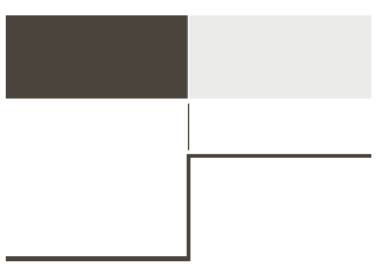
\includegraphics[width=.4\linewidth]{step-edge.png}%
}
\end{minipage}
\item 
\begin{minipage}[t]{\linewidth}
\raggedright Ramp edge: \hspace{3cm}
\adjustbox{valign=t}{%
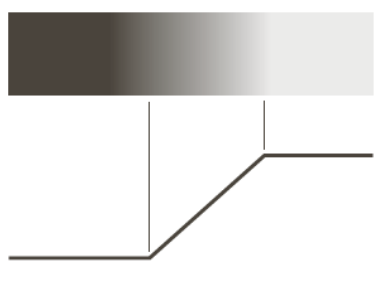
\includegraphics[width=.4\linewidth]{ramp-edge.png}%
}
\end{minipage}
\item 
\begin{minipage}[t]{\linewidth}
\raggedright Roof edge: \hspace{3cm}
\adjustbox{valign=t}{%
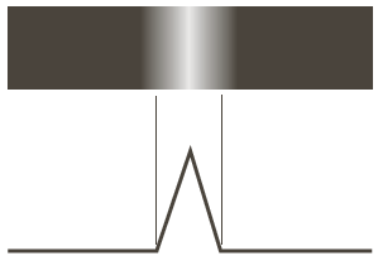
\includegraphics[width=.4\linewidth]{roof-edge.png}%
}
\end{minipage}
\end{itemize}
\pagebreak
Otherwise, edges can be affected by noise:
\begin{center}
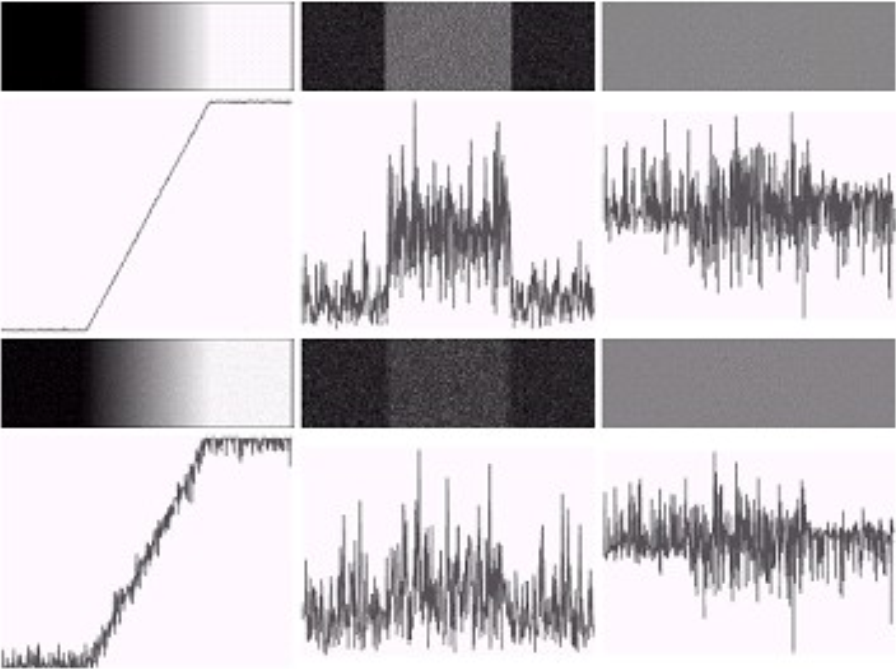
\includegraphics[width=\textwidth]{edge-noises.png}
\captionof{figure}{Edges with noise}
\end{center}
\subsubsection{Image derivative and edges:}
\subsubsection*{1.2.3.1 Image derivative:}
The first derivative ($gradient$) of the image is the base operator to measure edges in the image:
\begin{center}
$\mid \nabla f \mid \hspace{0.5cm} \equiv \Big( \frac{\partial f}{\partial x} \Big) ^2 \hspace{0.2cm} + \hspace{0.2cm} \Big(\frac{\partial f}{ \partial y}\Big)^2$
\end{center}
\begin{itemize}
\item 
\begin{minipage}[t]{\linewidth}
\raggedright Image histogram: \hspace{3cm}
\adjustbox{valign=t}{%
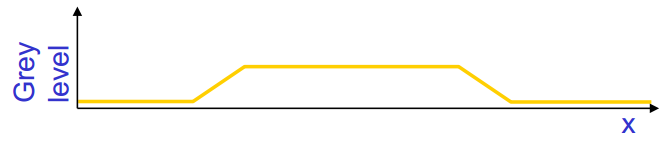
\includegraphics[width=.4\linewidth]{edge-histogram.png}%
}
\end{minipage}
\item 
\begin{minipage}[t]{\linewidth}
\raggedright First derivative $f'(x)$: \hspace{3cm}
\adjustbox{valign=t}{%
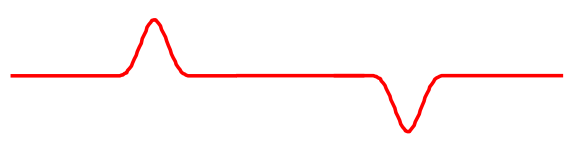
\includegraphics[width=.4\linewidth]{edge-1st-derivative.png}%
}
\end{minipage}
\item 
\begin{minipage}[t]{\linewidth}
\raggedright $\mid f'(x) \mid $  $\&$ threshold: \hspace{3cm}
\adjustbox{valign=t}{%
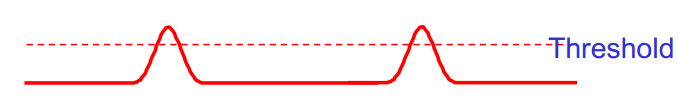
\includegraphics[width=.4\linewidth]{edge-2nd-derivative.png}%
}
\end{minipage}
\item 
\begin{minipage}[t]{\linewidth}
\raggedright $\mid f'(x) \mid $ $<$ threshold: \hspace{3cm}
\adjustbox{valign=t}{%
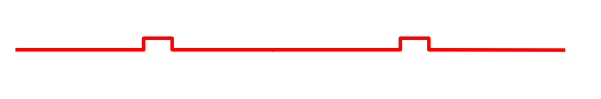
\includegraphics[width=.4\linewidth]{edge-filter.png}%
}
\end{minipage}
\end{itemize}
\pagebreak
\subsubsection{Filter/Kernel for detecting edges by convolution operation:}
\begin{itemize}
\item 
\begin{minipage}[t]{\linewidth}
\raggedright Roberts filter: \hspace{3cm}
\adjustbox{valign=t}{%
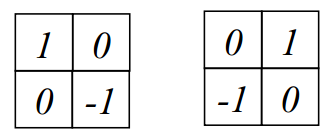
\includegraphics[width=.4\linewidth]{robert-filter.png}%
}
\end{minipage}
\item 
\begin{minipage}[t]{\linewidth}
\raggedright Sobel filter: \hspace{3cm}
\adjustbox{valign=t}{%
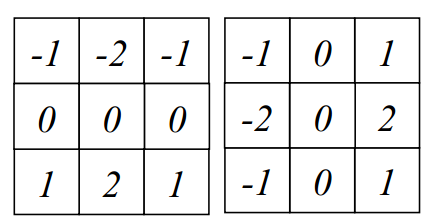
\includegraphics[width=.4\linewidth]{sobel-filter.png}%
}
\end{minipage}
\item 
\begin{minipage}[t]{\linewidth}
\raggedright Prewitt: \hspace{3cm}
\adjustbox{valign=t}{%
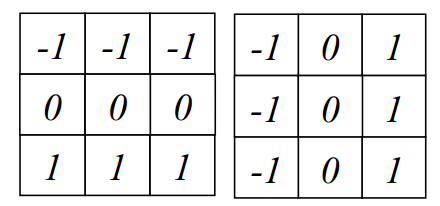
\includegraphics[width=.4\linewidth]{prewitt-filter.png}%
}
\end{minipage}
\end{itemize}
and etc...
\subsubsection{Image gradient:}
Derivative in X coordinate denoted as Gx, derivative in X coordinate denoted as Gy
\subsubsection*{1.2.5.1 Magnitude:}
Gradient intensity for each pixel:
\begin{center}
$
\mid G \mid \hspace{0.2cm} = \hspace{0.2cm} \sqrt{Gx^2 + Gy^2} \hspace{0.2cm} \approx \hspace{0.2cm} \mid Gx \mid \hspace{0.2cm} \mid Gy \mid 
$
\end{center}
\subsubsection*{1.2.5.2 Direction:}
Main gradient funtion for each pixel
\begin{center}
$
	\theta = arctan(Gy/Gx)
$
\end{center}
\subsubsection{Second image derivative}
Another approach to find edges in images is to use the \textit{second image derivative, for this, we use the $Laplacian$ as an operator}
\begin{center}
$
	\nabla ^ 2 I = \frac{\partial I}{\partial x ^2} + \frac{\partial I}{\partial y^2}
$
\end{center}
\subsubsection*{1.2.6.1 Laplacian using convolution:}
\begin{itemize}
\item Many discrete approximations exist for the Laplacian:
\[
  \begin{bmatrix}
    0 & 1 & 0\\
    1 & -4 & 1 \\
    0 & 1 & 0
  \end{bmatrix}
  \hspace{3cm}
    \begin{bmatrix}
    0 & 1 & 0\\
    1 & -8 & 1 \\
    0 & 1 & 0
  \end{bmatrix}
\]
\item One sole convolution matrix
\item Rotation symmetric
\end{itemize}
\subsubsection{Canny filter:}
Optimal filter for edge detection: filtering the image in several steps.\\ \par 
\subsubsection*{1.2.7.1.\hspace{0.5cm}Steps:}
\begin{enumerate}
\item Apply a Gaussian low-pass filter to remove noise on the image. 
\item Apply Sobel filter to the image and compute the gradient intensity and gradient direction in the image.
\item Non-maxima suppression: if the gradient magnitude of a pixel (x,y) is inferior to the one of its 2 neighbors along the gradient direction, then set this magnitude for (x,y) to zero.
\item Edge thressholding (hysteresis)
\begin{enumerate}
\item Use two thresholds: a threshold high (Sh) and a threshold low (Sb)
\item For each pixel in the gradient magnitude:
\begin{enumerate}
\item if $magnitude(x,y) < Sb$, then set this pixel to zero
\item If $magnitude(x,y) > Sh$, the set this pixel to edge pixel.
\item If $Sb < magnitude(x,y) \leq Sh$, then the pixel is set to edge pixel if it is connected to another edge pixel
\end{enumerate}
\end{enumerate}
\end{enumerate}
\subsection{Segmentation and Texture:}
\subsubsection{Segmentation:}
\subsubsection*{1.3.1.1\hspace{0.5cm}Definition:}
Segmentation aims to split an image into several parts which should correspond to object in the image
\subsubsection*{1.3.1.2\hspace{0.5cm} Goals:} 
Extract, separate elements in the image for applying a specific processing afterward or interpreting the image content.
\begin{itemize}
\item Discontinuities, edges: sudden changes, borders (frontier) between regions...
\item Homogeneous zones, regions: which has same colors, texture, intensity.
\end{itemize}
\subsubsection*{1.3.1.3\hspace{0.5cm}Methods:}
\begin{enumerate}
\item Thresholding
\begin{enumerate}
\item Histogram thresholding
\item Global thresholding
\item Multi-thresholding
\item Global automatic thresholding
\item Adaptive thresholding
\end{enumerate}
\item K-means algorithm
\item Split-and-merge
\item Watershed
\end{enumerate}
\subsubsection{Textures:}
\subsubsection*{1.3.2.1\hspace{0.5cm}Definition:}
Texture can be defined as a region with variation of intensity or as a spatial organization of pixels.
\subsubsection*{1.3.2.2\hspace{0.5cm}Methods:}
\begin{enumerate}
\item First order statistics: statistics on histogram
\item Co-occurence matrices: searching patterns
\item Frequential analysis: Gabor filter
\end{enumerate}
The most difficult is to find a good presentation for each texture.
\subsubsection{Color:}
\subsubsection*{1.3.3.1\hspace{0.5cm}Introduction:}
\begin{itemize}
\item Each pixel contains information from a spectral bandwidth.
\item We obtain color images, for example, by taking 3 bands from visible spectrum.
\item Some devices exist to acquire signal from more bands (X-ray, infrared, radio, ...)
\begin{center}

\includegraphics[width=\textwidth]{color-spectrum.png}
\captionof{figure}{Color spectrum}
\end{center}
\end{itemize}
\pagebreak
\subsubsection*{1.3.3.2\hspace{0.5cm}Primary colors:}
\begin{itemize}
\item RGB: Color representation using primary colors Red-Green-Blue:Additive scheme for displaying on a screen
\item CMY: Color representation using primary colors Cyan-Magenta-Yellow
\begin{itemize}
\item Subtractive scheme for printing on paper
\item We subtract from white instead of adding to black like in RGB
\item CMY = 1 - RGB
\end{itemize}
\end{itemize}
\begin{center}
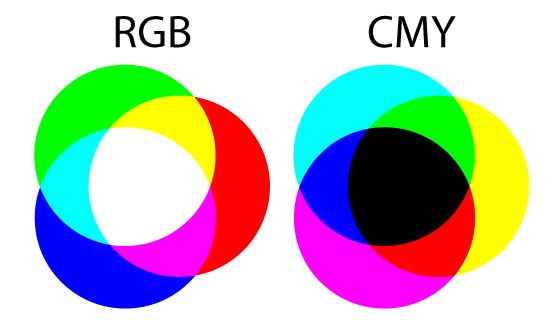
\includegraphics[width=\textwidth]{rgbCMY.png}
\captionof{figure}{RGB - CMY color space}
\end{center}
\subsubsection*{1.3.3.3\hspace{0.5cm}Color spaces}
\begin{itemize}
\item There are many different spaces to represent colors.
\item RGB is the most common color representation in computer. 
\item There are three types of color spaces:
\begin{itemize}
\item Purely physic approach
\item Purely visual approach
\item Physic approach but corrected by psychometry
\end{itemize}
\end{itemize}
\subsubsection*{1.3.3.4\hspace{0.5cm}HSV representation:}
\begin{center}
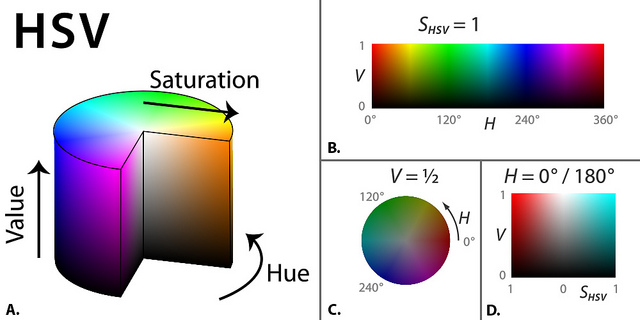
\includegraphics[width=\textwidth]{hsv_colorspace.jpg}
\captionof{figure}{HSV color space}
\end{center}
\begin{itemize}
\item H-Hue is coded as an angle between 0 and 360$^{\circ}$
\item S-Saturation is coded as a radius between 0 and 1, S = 0 $\sim$ gray, S = 1 $\sim$ pure color
\item V-Value = MAX(Red, Green, Blue)
\end{itemize}
\section{Operations and Transformations:}
\subsection{Operations:}
\subsubsection{Contrast enhancement:}
\begin{itemize}
\item Linear Transformation: Enhance the dynamic range by linearly stretching the original gray levels to the range of target.
\item Piecewise Linear Transformation: Linear stretching with k segments.
\item Non-linear Transformation:
\begin{itemize}
\item Non-linear functions with a fixed form.
\item Fewer parameters to adjust.
\item Satisfying: $ 0 = f_{min} \leq g \leq f_{max} = L - 1$
\item Examples:
\begin{itemize}
\item Logarithmic transformation: stretch dark region, suppress bright region
\begin{center}
$ g = b.log(af +1) $
\end{center}
\item Exponential transformation: expand bright region
\begin{center}
$ g = b(e^{af} -1) $
\end{center}
\item Power law: $ g = af^k$\\
$k = 2$: square law, similar to exponential, $k = \frac{1}{3}$: cubic root, similar to logarithmic
\end{itemize}
\end{itemize}
\item Histogram Equalization:
Transform an image with arbitrary histogram to one with a flat histogram
\begin{itemize}
\item Suppose $f$ has PDF $p_F(f), 0 \leq f \leq 1$
\item Transform function (continuous): $g(f) = \int_{0}^{f}p_F(t)dt$
\end{itemize}
\end{itemize}
\subsubsection{Image operators}
\begin{itemize}
\item Logical operators: AND, OR, XOR, NOT 
\item Addition, Subtraction, Multiplication: add, subtract, multiply two pixels in two images with the corresponding position with upperbound 255 and lowerbound 0 into a new values of new image.
\end{itemize}
\subsubsection{Interpolation}
\begin{itemize}
\item Nearest Neighbor Interpolation:\\
Interpolation uses the values of the nearby translated pixel for the output pixel values.
\item Bilinear Interpolation:\\
The block uses the weighted average of two translated pixel values for each output pixel value.
\item Bicubic Interpolation:\\
The block uses the weighted average of four translated pixel values for each output pixel value.
\end{itemize}
\subsection{Transformations}
\subsubsection{Fourier Transforms:}
\begin{itemize}
\item Fourier transforms applied in Image Processing is Discrete Fourier Transforms because spatial domain from image is discrete
\item The output of the transformation represents the image in the frequency domain.
\begin{center}
$
	f(x,y) = \int_{-\infty}^{\infty}\int_{-\infty}^{\infty}F(u,v)e^{j2\pi (ux+uy)}dudv
$
\end{center}
\begin{center}
$
    F(u,v) = \int_{-\infty}^{\infty}\int_{-\infty}^{\infty}f(x,y)e^{j2\pi (ux+uy)}dxdy
$
\end{center}
where $u$ and $v$ are spatial frequencies
\item Fourier transformation produces a complex number valued output image. We use the real part to represent geometric structure of the spatial domain image. However, we need the real and the imaginary part to re-transform the image.
\begin{itemize}
\item $F(u,v)$ is complex in general
\begin{center}
$
	F(u,v) = F_R(u,v) + jF_i(u,v)
$
\end{center}
\item $\mid F(u,v)\mid$ is the magnitude spectrum
\item $\arctan(F_i(u,v)/F_R(u,v))$ is the phase angle spectrum
\end{itemize}
\item High frequencies: The points far from from FT center.
\item Low frequencies: The points near from FT center
\item Applications: Image analysis, image filtering, image reconstruction and image compression
\end{itemize}
\subsubsection{Hough transforms:}
\begin{itemize}
\item Hough transformation can be used to detect lines circles of used to detect other parametric curves.
\item It can give robust detection under noise and partial occlusion.
\item Transform line in $x-y$ space to point in $m-c$ space:
\begin{center}
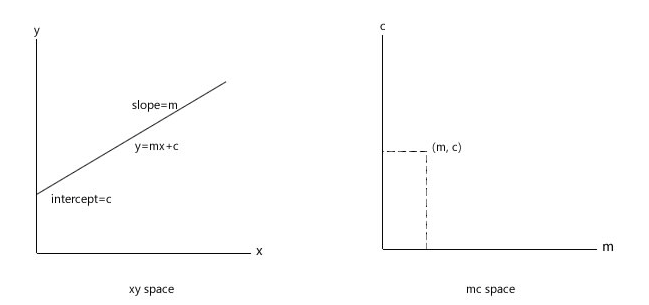
\includegraphics[scale=0.4]{xy-mc.png}
\captionof{figure}{Line in xy space to point in mc space}
\end{center}
\item Transform point in $x-y$ space to line in $m-c$ space:
\begin{center}
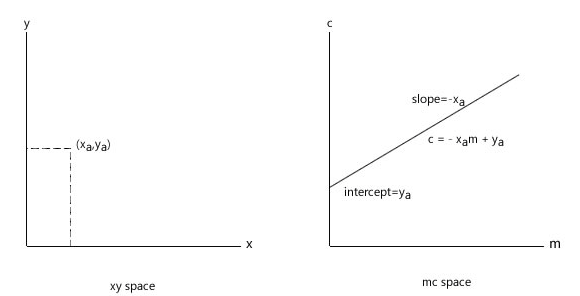
\includegraphics[scale=0.4]{xy-mc-point.png}
\captionof{figure}{Point in xy space to line in mc space}
\end{center}
\item For Hough transform, taken an edge detected image, for every point that is non-black, draw lines in the $m-c$ space. Obviously, some lines will intersect. These intersections mark are the parameters of the line.
\begin{center}
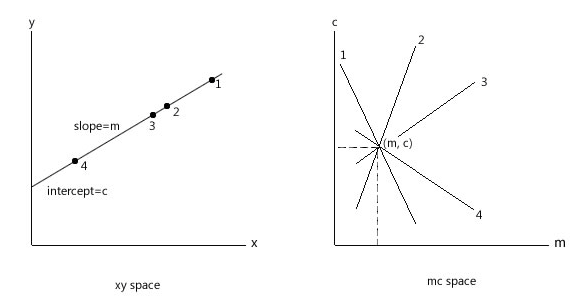
\includegraphics[width=\textwidth]{xy-mc-example.png}
\captionof{figure}{Lines and points in xy space to points and lines in mc space}
\end{center}
\end{itemize}
\section{SIFT \& SURF:}
\subsection{SIFT}
\subsubsection{Description:}
The scale invariant feature transform, SIFT [17], extracts a set of descriptors from an image. The
extracted descriptors are invariant to image translation, rotation and scaling (zoom-out). SIFT
descriptors have also proved to be robust to a wide family of image transformations, such as slight
changes of viewpoint, noise, blur, contrast changes, scene deformation, while remaining discriminative
enough for matching purposes
\subsubsection{Algorithm:}
\begin{enumerate}
\item Compute the Gaussian scale-space defined as function $L(x,y,\sigma)$ with the variable-scale Gaussian $G(x,y,\sigma)$ and the input image $I(x,y)$: 
\begin{center}
$
	L(x,y,\sigma) = G(x,y,\sigma) * I(x,y)
$
\end{center}
where $*$ is convolution operation in x and y and $G(x,y,\sigma) = \frac{1}{2\pi \sigma^2}e^{-\frac{x^2+y^2}{2\sigma^2}} $
\item compute the Difference of Gaussians(DoG)
\begin{center}
$
	D(x,y,\sigma) = L(x,y,k\sigma) - L(x,y,\sigma)
$
\end{center}
\item Find candicate keypoints (3D discrete extrema of DoG) by comparing a pixel to its 26 neighbors in 3x3 regions at the current and adjacent scales.
\item Refine candicate keypoints location with sub-pixel precision.
\item Filter unstable keypoints due to noise.
\item Filter unstable keypoints lying on edge using Taylor expansion of scale-space function.
\item Assign a reference orientation to each keypoint based on scale-space gradient and orientation.
\item Build the keypoints d;escriptor ${(x,y,\sigma,\theta,\textbf{f})}$
\end{enumerate}
\subsection{SURF}
\subsubsection{Introduction:}
In computer vision, speeded up robust features (SURF) is a patented local feature detector and descriptor. It can be used for tasks such as object recognition, image registration, classification or 3D reconstruction. It is partly inspired by the scale-invariant feature transform (SIFT) descriptor
\subsubsection{Algorithm:}
To detect interest points, SURF uses an integer approximation of the determinant of Hessian blob detector, which can be computed with 3 integer operations using a precomputed integral image. Its feature descriptor is based on the sum of the Haar wavelet response around the point of interest. These can also be computed with the aid of the integral image.

SURF descriptors have been used to locate and recognize objects, people or faces, to reconstruct 3D scenes, to track objects and to extract points of interest.
\subsection{Comparison:}
\begin{enumerate}
\item Change of Viewpoint:
\begin{center}
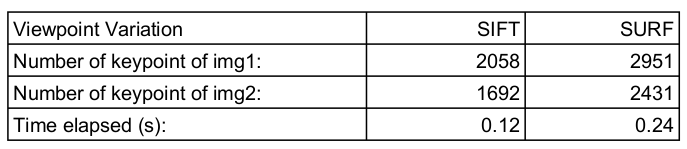
\includegraphics[scale=0.3]{viewpoint.png}
\end{center}
\item Salt-pepper noise with rate of 0.5:
\begin{center}
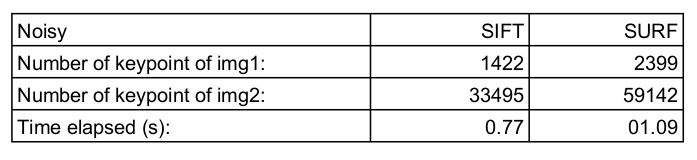
\includegraphics[scale=0.3]{noisy.png}
\end{center}
\item Angle Variation of 45 $^{\circ}$:
\begin{center}
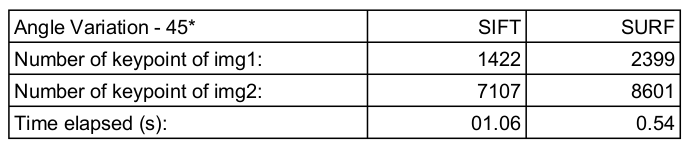
\includegraphics[scale=0.3]{angle-45.png}
\end{center}
\item Angle Variation of 90 $^{\circ}$:
\begin{center}
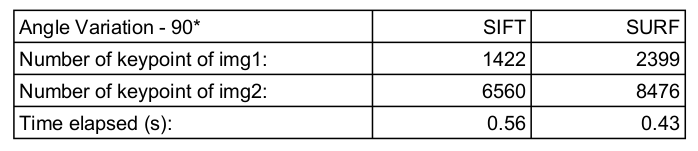
\includegraphics[scale=0.3]{angle-90.png}
\end{center}
\item Angle Variation of 135 $^{\circ}$:
\begin{center}
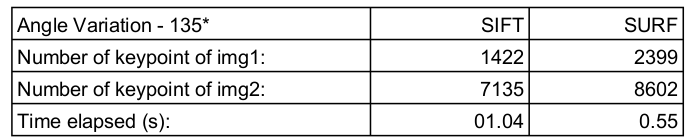
\includegraphics[scale=0.3]{angle-135.png}
\end{center}
\item Angle Variation of 180 $^{\circ}$:
\begin{center}
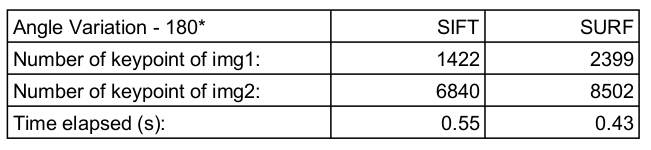
\includegraphics[scale=0.3]{angle-180.png}
\end{center}
\end{enumerate}



\section{Neural Network in Computer Vision:}
\subsection{Neural Network:}
\subsubsection{Definitions:}
An Artificial Neural Network is an information processing paradigm that is inspired by the way biological nervous system, such as brain, process information. The key element of this paradigm is the novel structure of the information processing system. It is composed of a large number of highly interconnected processing elements (neurones) working in unison to solve specific problems. ANNs, like people, learn by example. An ANN is configured for a specific application, such as pattern recognition or data classification, through a learning process. Learning in biological systems involves adjustments to the synaptic connections that exist between the neurones
\subsubsection{Architecture:}

Neural Network as neurons in graphs. Neural Networks are modeled as collections of neurons that are connected in an acyclic graph. In other words, the outputs of some neurons can become inputs to other neurons.
\begin{center}
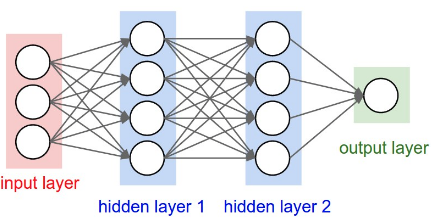
\includegraphics[width=\textwidth]{nn-architecture.png}
\captionof{figure}{Neural Network with 2 hidden layers}
\end{center}
\begin{enumerate}
\item Input layer: this is the first layer of a neural network. It is used to provide the input data or features to the network
\item Output layer. Unlike all layers in a Neural Network, the output layer neurons most commonly do not have an activation function (or you can think of them as having a linear identity activation function). This is because the last output layer is usually taken to represent the class scores (e.g. in classification), which are arbitrary real-valued numbers, or some kind of real-valued target (e.g. in regression).
\item Hidden layer: A feedforward network applies a series of functions to the input. By having multiple hidden layers, we can compute complex functions by cascading simpler functions. The number of hidden layers is termed as the depth of the neural network. In general, deeper networks can learn more complex functions.
\end{enumerate}
\subsubsection{Activation Functions}
\begin{enumerate}
\item Sigmoid functions: It maps the input ($x$ axis) to values between 0 and 1.
\begin{center}
$
	\sigma(x) = \frac{1}{1+e^{-x}}
$
\end{center}
\begin{center}
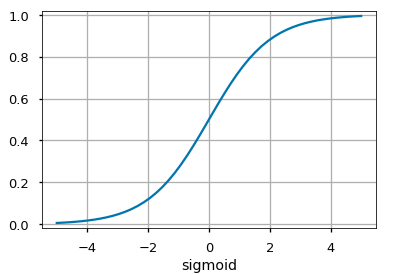
\includegraphics[scale=0.5]{nn-sigmoid.png}
\captionof{figure}{sigmoid function}
\end{center}
In practice, the sigmoid non-linearity has recently fallen out of favor and it is rarely ever used. It has two major drawbacks:
\begin{itemize}
\item Sigmoid saturates and kills gradients: when the neuron’s activation saturates at either tail of 0 or 1, the gradient at these regions is almost zero. Therefore, if the local gradient is very small, it will effectively “kill” the gradient and almost no signal will flow through the neuron to its weights and recursively to its data.
\item Sigmoid outputs are not zero-centered:This has implications on the dynamics during gradient descent, because if the data coming into a neuron is always positive (e.g. $x>0$ elementwise in $f=wTx+b$)), then the gradient on the weights $w$ will during backpropagation become either all be positive, or all negative (depending on the gradient of the whole expression $f$). This could introduce undesirable zig-zagging dynamics in the gradient updates for the weights.
\end{itemize}
\item Tanh functions:It is similar to the sigmoid function butmaps the input to values between -1 and 1.
\begin{center}
$
	\tanh(x)=2\sigma(2x)−1 .
$
\end{center}
\begin{center}
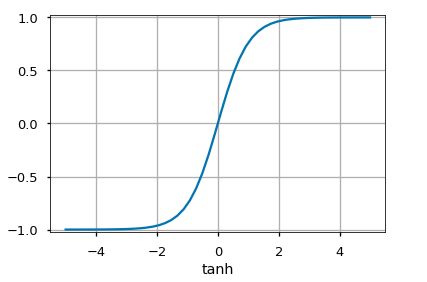
\includegraphics[scale=0.5]{nn_tanh.png}
\captionof{figure}{tanh function}
\end{center}
Like the sigmoid neuron, its activations saturate, but unlike the sigmoid neuron its output is zero-centered. Therefore, in practice the tanh non-linearity is always preferred to the sigmoid nonlinearity.
\pagebreak
\item Rectified Linear Unit(ReLU): It allows only positive values to pass through it. The negative values are mapped to zero.
\begin{center}
$
	f(x)=\max(0,x)
$
\end{center}
\begin{center}
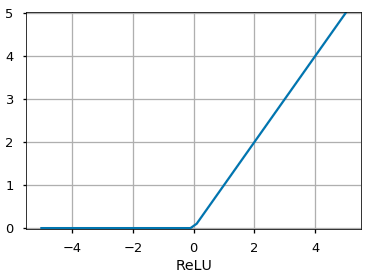
\includegraphics[scale=0.5]{nn-relu.png}
\captionof{figure}{ReLU function}
\end{center}
\begin{enumerate}
\item Advantages:
\begin{itemize}
\item It was found to greatly accelerate the convergence of stochastic gradient descent compared to the sigmoid/tanh functions.
\item  Compared to tanh/sigmoid neurons that involve expensive operations (exponentials, etc.), the ReLU can be implemented by simply thresholding a matrix of activations at zero.
\end{itemize}
\item Disadvantages:
\begin{itemize}
\item  ReLU units can be fragile during training and can “die”. For example, a large gradient flowing through a ReLU neuron could cause the weights to update in such a way that the neuron will never activate on any datapoint again. If this happens, then the gradient flowing through the unit will forever be zero from that point on
\end{itemize}
\end{enumerate}
\end{enumerate}
\pagebreak
\subsubsection{Optimization:}
\begin{center}
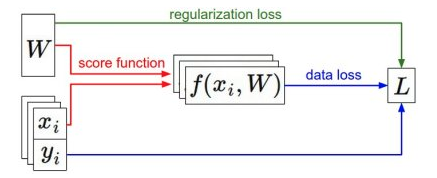
\includegraphics[width=\textwidth]{nn-optimization.png}
\captionof{figure}{Optimization}
\end{center}
The dataset of pairs of $(x,y)$ is given and fixed. The weights start out as random numbers and can change. During the forward pass the score function computes class scores, stored in vector $f$. The loss function contains two components: The data loss computes the compatibility between the scores $f$ and the labels $y$. The regularization loss is only a function of the weights. During Gradient Descent, we compute the gradient on the weights (and optionally on data if we wish) and use them to perform a parameter update during Gradient Descent.
\subsubsection{Backpropagation:}
A way of computing gradients of expressions through recursive application of chain rule.Our goal with backpropagation is to update each of the weights in the network so that they cause the actual output to be closer the target output, thereby minimizing the error for each output neuron and the network as a whole.
\subsection{Convolution Neural Network:}
\subsubsection{Definition:}
Convolutional Neural Networks are very similar to ordinary Neural Networks: they are made up of neurons that have learnable weights and biases. Each neuron receives some inputs, performs a dot product and optionally follows it with a non-linearity. The whole network still expresses a single differentiable score function: from the raw image pixels on one end to class scores at the other. And they still have a loss function (e.g. SVM/Softmax) on the last (fully-connected) layer and all the tips/tricks we developed for learning regular Neural Networks still apply
\subsubsection{Why Convolution Neural Network in Computer Vision:}
Input images for processing in Computer Vision usually consist of 3 channel colors with size MxN pixels, for example in CIFAR10 data set each image is size of 32x32x3 $\approx$ 3072 weights. Clearly, full connectivity in Regular Neural Nets  is wasteful and the huge number of parameters would quickly lead to overfitting and cause very costly computational. While Convolutional Neural Networks take advantage of the fact that the input consists of images and they constrain the architecture in a more sensible way. In particular, unlike a regular Neural Network, the layers of a ConvNet have neurons arranged in 3 dimensions: width, height, depth. The neurons in a layer will only be connected to a small region of the layer before it, instead of all of the neurons in a fully-connected manner
\subsubsection{Architecture:}
\begin{itemize}
\item CONV layer will compute the output of neurons that are connected to local regions in the input, each computing a dot product between their weights and a small region they are connected to in the input volume. 
\item RELU layer will apply an element-wise activation function, such as the max(0,x) thresholding at zero. 
\item POOL layer will perform a down-sampling operation along the spatial dimensions (width, height).
\item FC (i.e. fully-connected) layer will compute the class scores. As with ordinary Neural Networks and as the name implies, each neuron in this layer will be connected to all the numbers in the previous volume.
\end{itemize}
\section{Projects:}
\subsection{Environments, dataset, frameworks:}
\subsubsection{Environments:}
\begin{itemize}
\item OS: Linux - Ubuntu 16.04
\item Programing Language: Python (3.5) - an interpreted high-level programing language, close to human language.
\end{itemize}
\subsubsection{Dataset:}
\begin{itemize}
\item CIFAR10: a dataset consists of 60000 32x32 colour images in 10 classes, with 6000 images per class. There are 50000 training images and 10000 test images used for Classification.
\item Object images: high-resolution image of object to identify the error on it.
\end{itemize}
\subsubsection{Frameworks:}
\begin{itemize}
\item Anaconda: Free, open-source packages management and deployment aimed distribution of Python.
\item Scientific Python distributions: Numpy, Scipy, Matplotlib, ipython, jupyter, Pandas, SciKit learn.
\item Pytorch: a python package that provides two high-level features:
\begin{itemize}
\item Tensor computation (like Numpy) with strong GPU acceleration
\item Deep Neural Networks built on a tape-based autodiff system. 
\end{itemize}
\item OpenCV-Python: (Open Source Computer Vision Library) is an open source computer vision and machine learning software library. 
\end{itemize}
\subsection{Image Classification with CIFAR10 dataset:}
\subsubsection{Self-made convolution network:}
A simple Convolution Network with 3 CONV layers with MaxPooling layers, 3 FC layers and the the ReLu activation function was made to understand roles of each layer in CNN and how to implement a CNN in Pytorch.
\begin{itemize}
\item Models: \begin{itemize}
\item conv layer 1: $Conv2d(3, 12, kernel\_size=(5, 5), stride=(1, 1), padding=(2, 2))$
\item pool layer: $MaxPool2d(kernel\_size=2, stride=2, padding=0, dilation=1, ceil\_mode=False)$
\item conv layer 2: $Conv2d(12, 18, kernel\_size=(5, 5), stride=(1, 1), padding=(2, 2))$
\item pool layer: $MaxPool2d(kernel\_size=2, stride=2, padding=0, dilation=1, ceil\_mode=False)$
\item conv layer 3: $Conv2d(18, 26, kernel\_size=(3, 3), stride=(1, 1))$
\item pool layer: $MaxPool2d(kernel\_size=2, stride=2, padding=0, dilation=1, ceil\_mode=False)$
\item fc layer 1: $Linear(in\_features=234, out\_features=200, bias=True)$
\item fc layer 2: $Linear(in\_features=200, out\_features=84, bias=True)$
\item fc layer 3: $Linear(in\_features=84, out\_features=10, bias=True)$
\end{itemize}
With the ReLU activation function
\item Train loss: 1.547 and Accuracy: 45.96$\%$
\item Test loss: 1.335 and Accuracy: 54.740$\%$
\end{itemize}
\subsubsection{Residual Network (a.k.a ResNet):}
\subsubsection*{5.2.2.1\hspace{0.5cm}Why Residual Network?}
When Microsoft Research released Deep Residual Learning for Image Recognition in 2015, these networks led to 1st-place winning entries in all five main tracks of the ImageNet and COCO 2015 competitions, which covered image classification, object detection, and semantic segmentation. The robustness of ResNets has since been proven by various visual recognition tasks and by non-visual tasks involving speech and language.\\
\pagebreak
\par
Deep networks are hard to train because of the notorious vanishing or exploding gradient problem - as the gradient is back-propagated to earlier layers, repeated multiplication may make the gradient infinitively small. As a result, as the network goes deeper, its performance gets saturated or even starts degrading rapidly.
\begin{center}
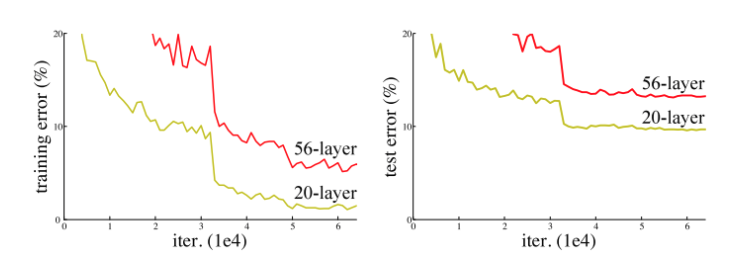
\includegraphics[width=\textwidth]{train-test-error.png}
\captionof{figure}{Increasing network depth leads to worse performance}
\end{center}

\par The core idea of ResNet to tackle vanishing the above problems is introducing a so-called “identity shortcut connection” that skips one or more layers, as shown in the following figure:
\begin{center}
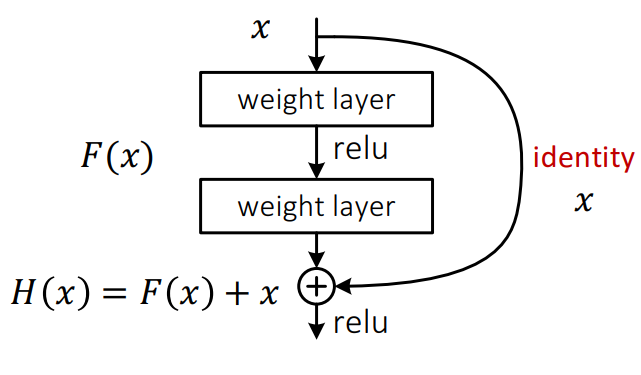
\includegraphics[width=\textwidth]{skip_connection.png}
\captionof{figure}{A residual block}
\end{center}
Skip connections which allows you to take the activation from one layer and suddenly feed it to another layer even much deeper in the neural network. And using that, ResNet enables to train very, very deep networks. \par
Instead of learning a direct mapping of $x->y$ with a function $H(x)$. Let define the residual function using $F(x) = H(x) - x$, which can be reframed into $H(x) = F(x)+x$, where $F(x)$ and $x$ represent the stacked non-linear layers and the identity function respectively. The author's hypothesis is that it is easy to optimize the residual mapping function $F(x)$ than to optimize the original, unreferenced mapping $H(x)$.
\pagebreak
\par The authors of [2] argue that stacking layers shouldn’t degrade the network performance, because we could simply stack identity mappings (layer that doesn’t do anything) upon the current network, and the resulting architecture would perform the same. This indicates that the deeper model should not produce a training error higher than its shallower counterparts. They hypothesize that letting the stacked layers fit a residual mapping is easier than letting them directly fit the desired underlaying mapping. And the residual block above explicitly allows it to do precisely that.
\begin{center}
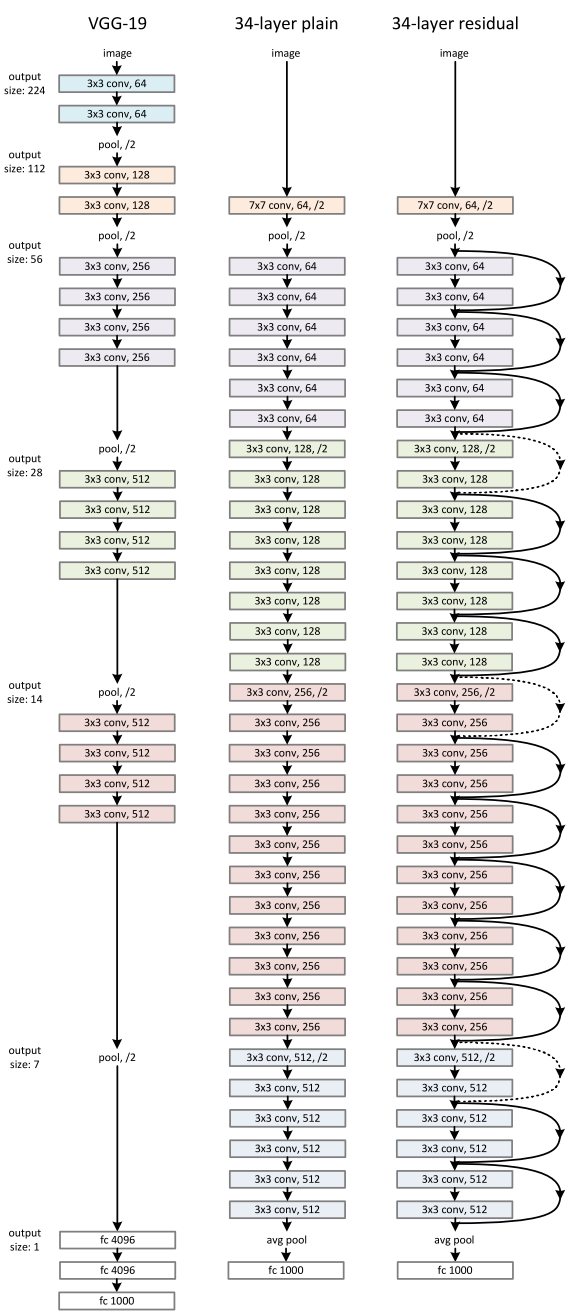
\includegraphics[scale=0.3]{compare_resnet.png}
\captionof{figure}{ResNet Architecture}
\end{center}
\pagebreak
\par Furthermore, in ResNet, the authors proposed using Batch Normalization which also helps the network to solve vanishing gradients problem.
\begin{itemize}
\item Address the problem of vanishing/exploding gradients
\item Increase learning speed and solve many other problems
\item Each activation in every iteration each layer is normalized to have zero mean and variance 1 over a minibatch
\item Integrated into back-propagation algorithm
\end{itemize}
Batch Normalization:
\begin{itemize}
\item \textbf{Input:}Value of $x$ over a mini-batch $ B = \{ x_{1...m} \} $. Parameters to be learned: $\gamma, \beta$\\
\item \textbf{Output:}$ \{y_i = BN_{\gamma, \beta}(x_i)\}$
\begin{itemize}
\item Mini-batch mean:\hspace{0.2cm}$\mu_B \leftarrow \frac{1}{m}\Sigma^m_{i=1}x_i$\\[0.2cm]
\item Mini-batch variance:\hspace{0.2cm}$\sigma^2_B \leftarrow \frac{1}{m}\Sigma^m_{i=1}(x_i-\mu_B)^2 $\\[0.2cm]
\item Normalize:\hspace{0.2cm}$\hat{x_i} \leftarrow \frac{x_i - \mu_B}{\sqrt{\sigma^2_B + \epsilon}}$\\[0.2cm]
\item Scale and shift:\hspace{0.2cm}$y_i \leftarrow \gamma \hat{x_i} + \beta \equiv BN_{\gamma, \beta}(x_i) $
\end{itemize}
\end{itemize}
\subsubsection*{5.2.2.2\hspace{0.5cm}ResNet 34:}
To execute classification on CIFAR10 dataset, I would like to use ResNet 34 architecture in Residual Network framework. Due to availability on my own hardware to develop and debug and the experimental errors on the ImageNet data set.
\begin{center}
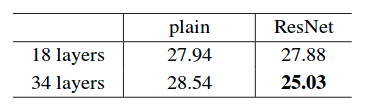
\includegraphics[scale=0.5]{image-net_err.png}
\captionof{figure}{Top-1 error($\%$, 10-crop testing)} on ImageNet validation.
\end{center}
\pagebreak
Intuitively, We have the architecture of the ResNets including ResNet 34.
\begin{center}
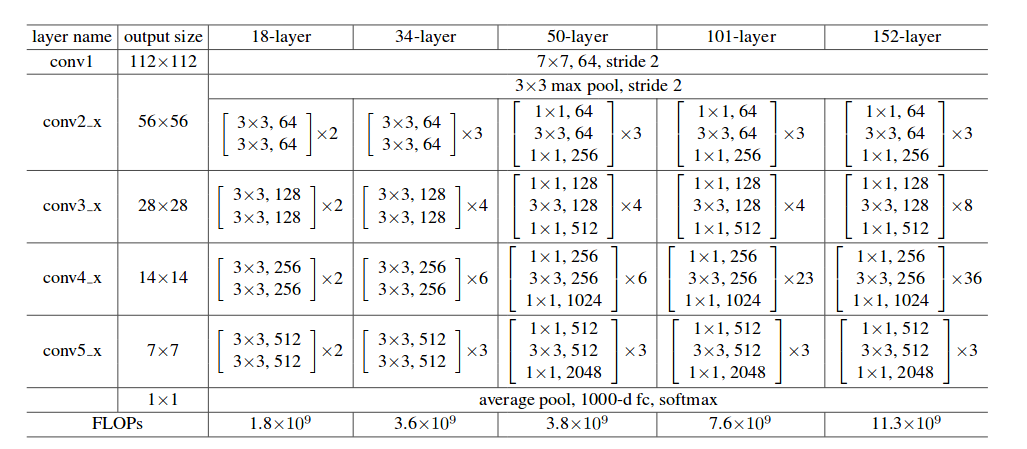
\includegraphics[width=\textwidth]{resnet-architecture.png}
\captionof{figure}{ResNets architecture}
\end{center}
\subsubsection*{5.2.2.3\hspace{0.5cm}Implementation and Results:}
\hspace{0.2cm} The code of this project has been public on Github: \\
\begin{center}
\url{https://github.com/t3min4l/pytorch-cifar10}
\end{center}
\par Result with 150 epochs, learning-rate: 0.1:\\ Best accuracy on Test set: 87.98\% while loss is 0.35
\subsubsection{Error detection on object in image:}
\subsubsection*{5.2.3.1\hspace{0.5cm}Propose idea:}
\begin{enumerate}
\item Find contour of the objects
\item Find minReact contain the contour
\item Find centroid of contour, and apply perspective transform
\item Draw midperpendiculars of the contour and split images in half
\item Detect differences by using function `compare$\_$ssim' from `skimage'
\end{enumerate}
\pagebreak
\subsubsection*{5.2.3.3\hspace{0.5cm}Execution:}
\begin{enumerate}
\item Find contour of the object:
\begin{enumerate}
\item Convert color from RGB to gray
\begin{center}
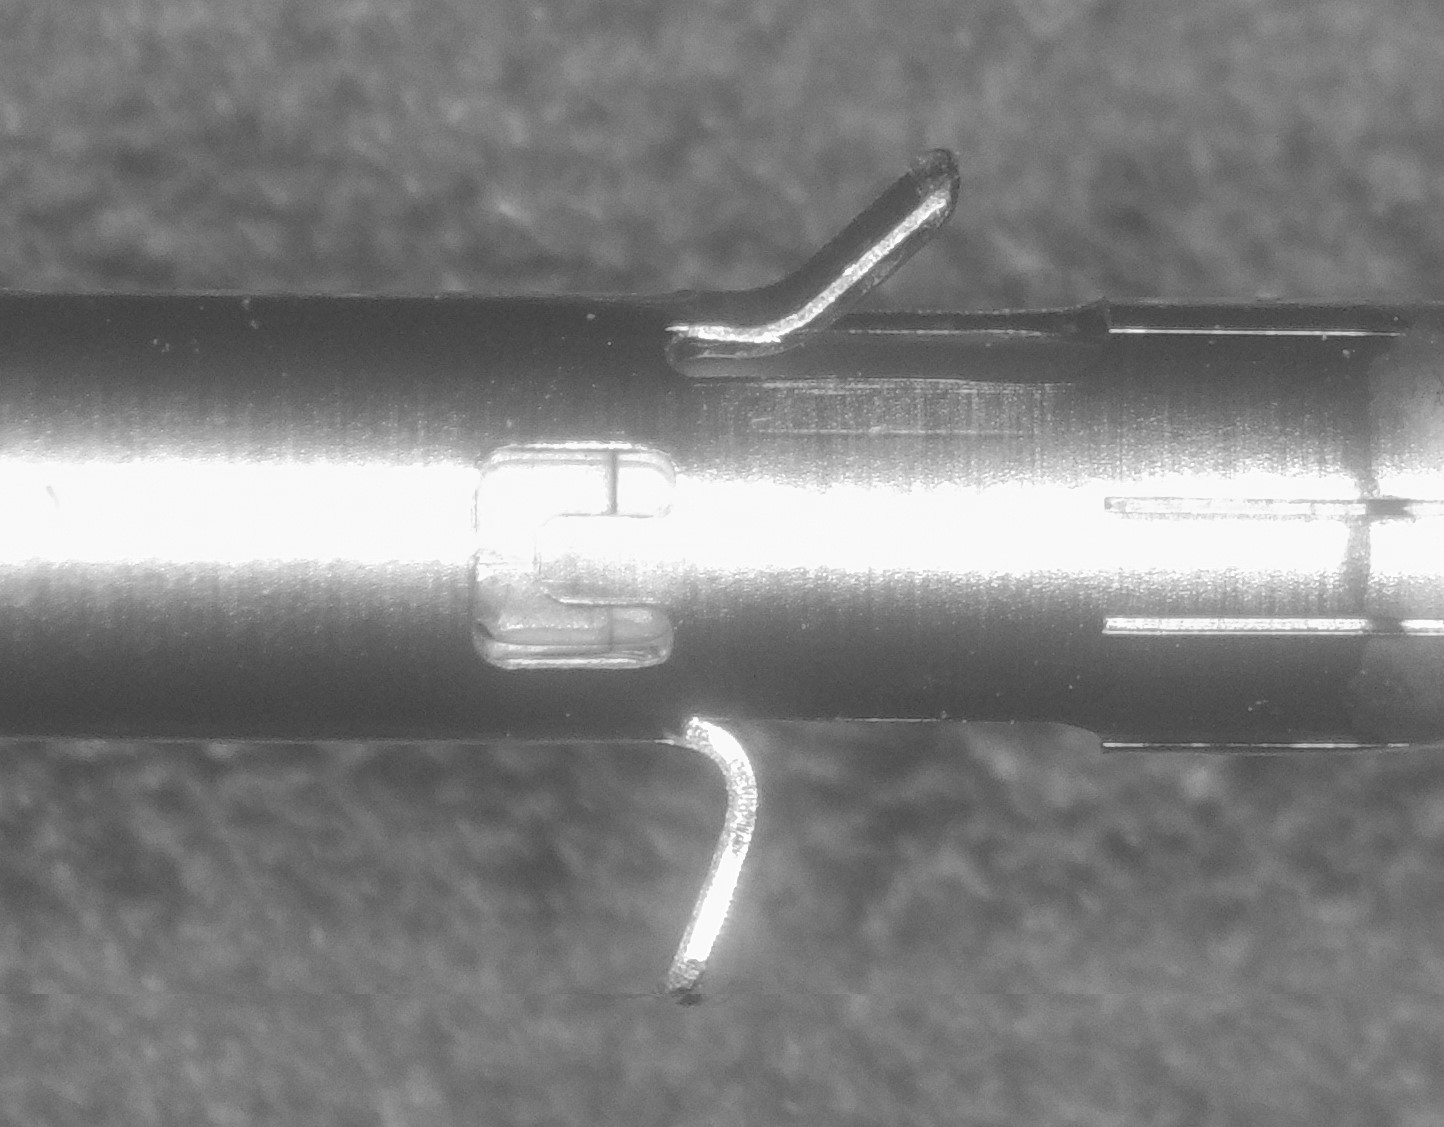
\includegraphics[width=\textwidth]{grayed.png}
\captionof{figure}{Convert image to gray scale}
\end{center}
\pagebreak
\item Apply Canny edge detector
\begin{center}
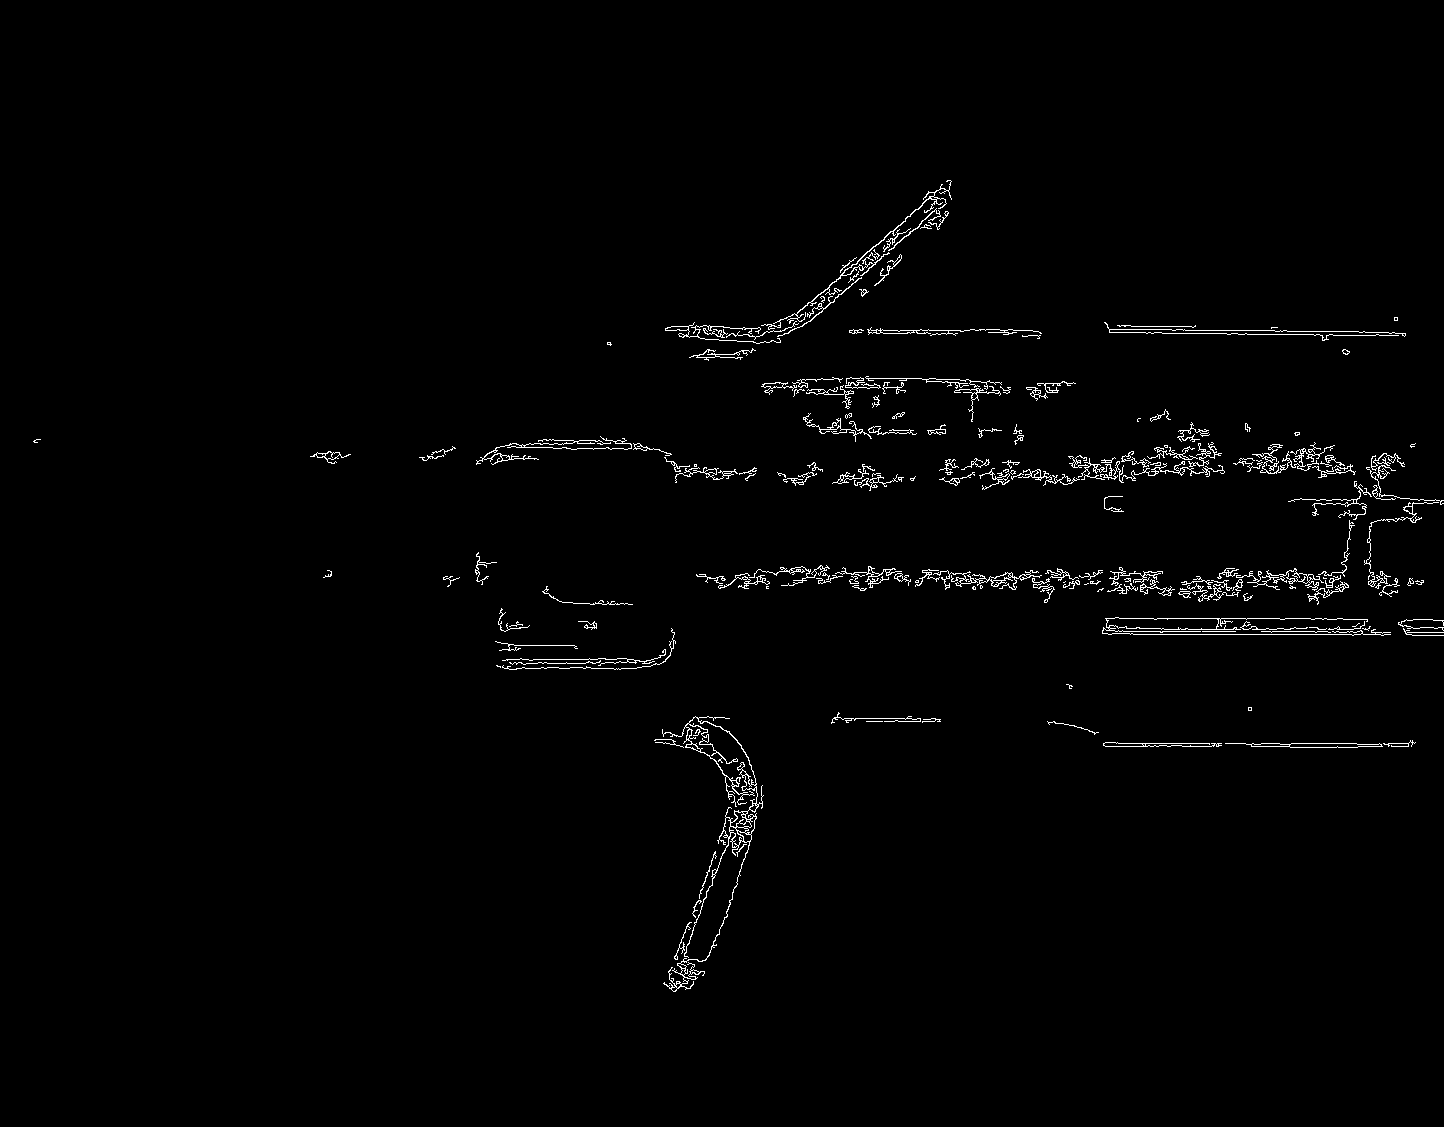
\includegraphics[width=\textwidth]{edged.png}
\captionof{figure}{Edges detected by Canny algorithm}
\end{center}
\pagebreak
\item Apply Morphological transformation
\begin{center}
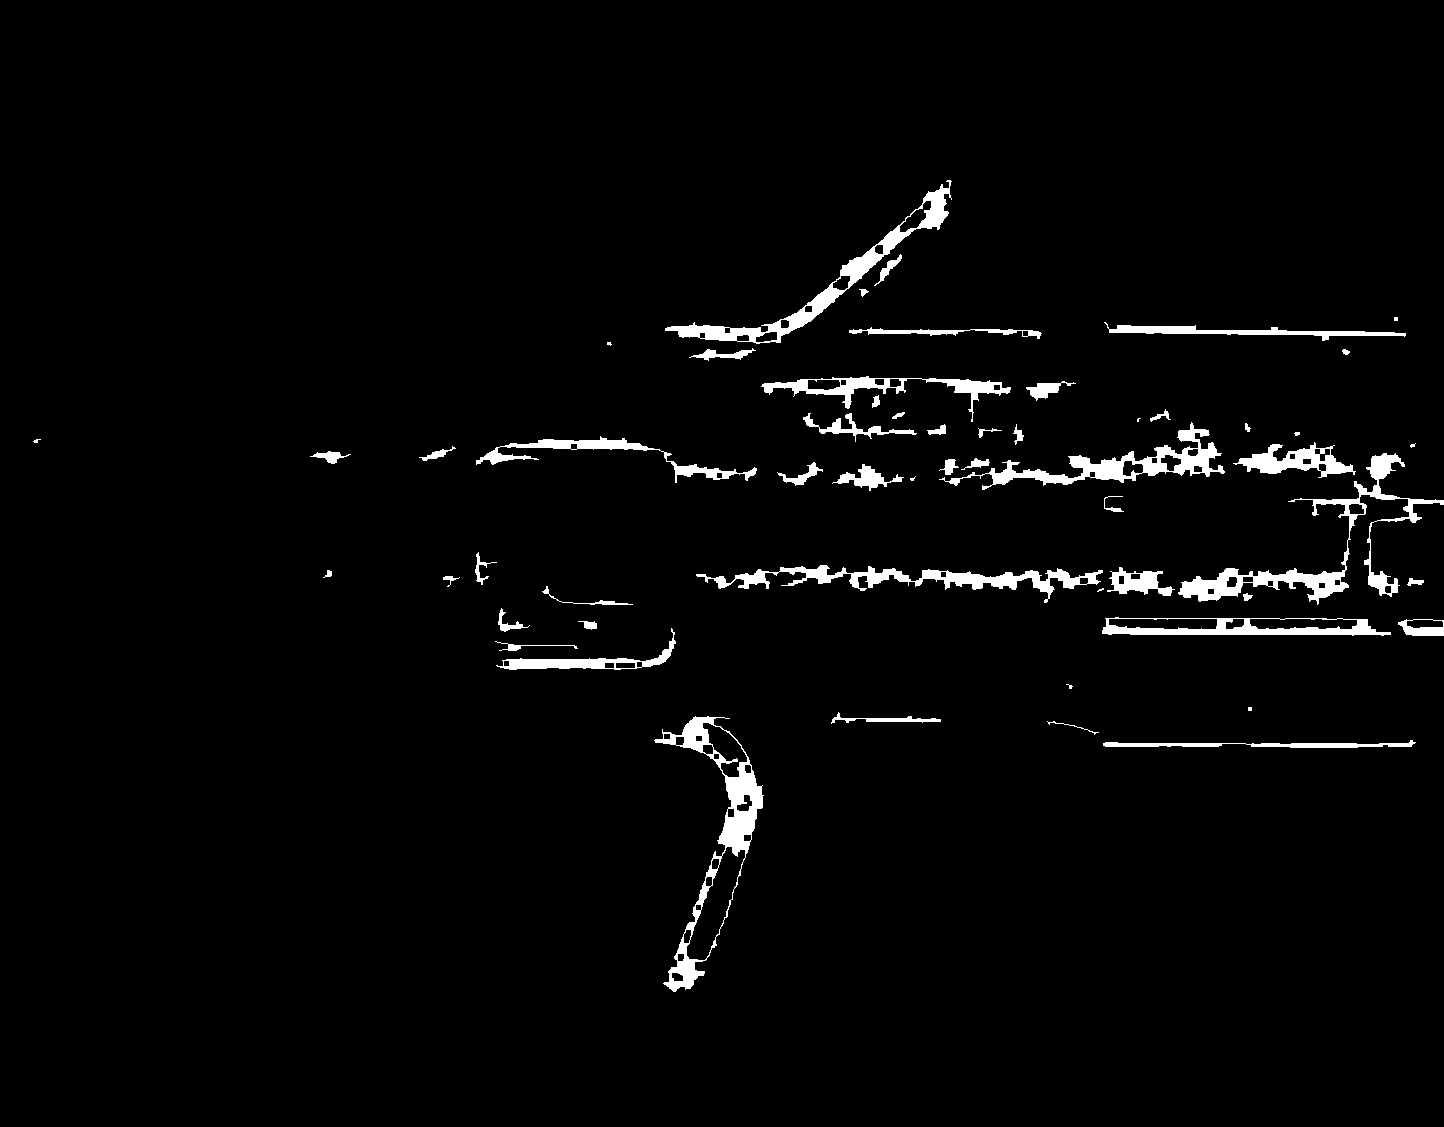
\includegraphics[width=\textwidth]{mophor.png}
\captionof{figure}{Morphological gradients transformation}
\end{center}
\pagebreak
\item Find contours and draw them on the image
\begin{center}
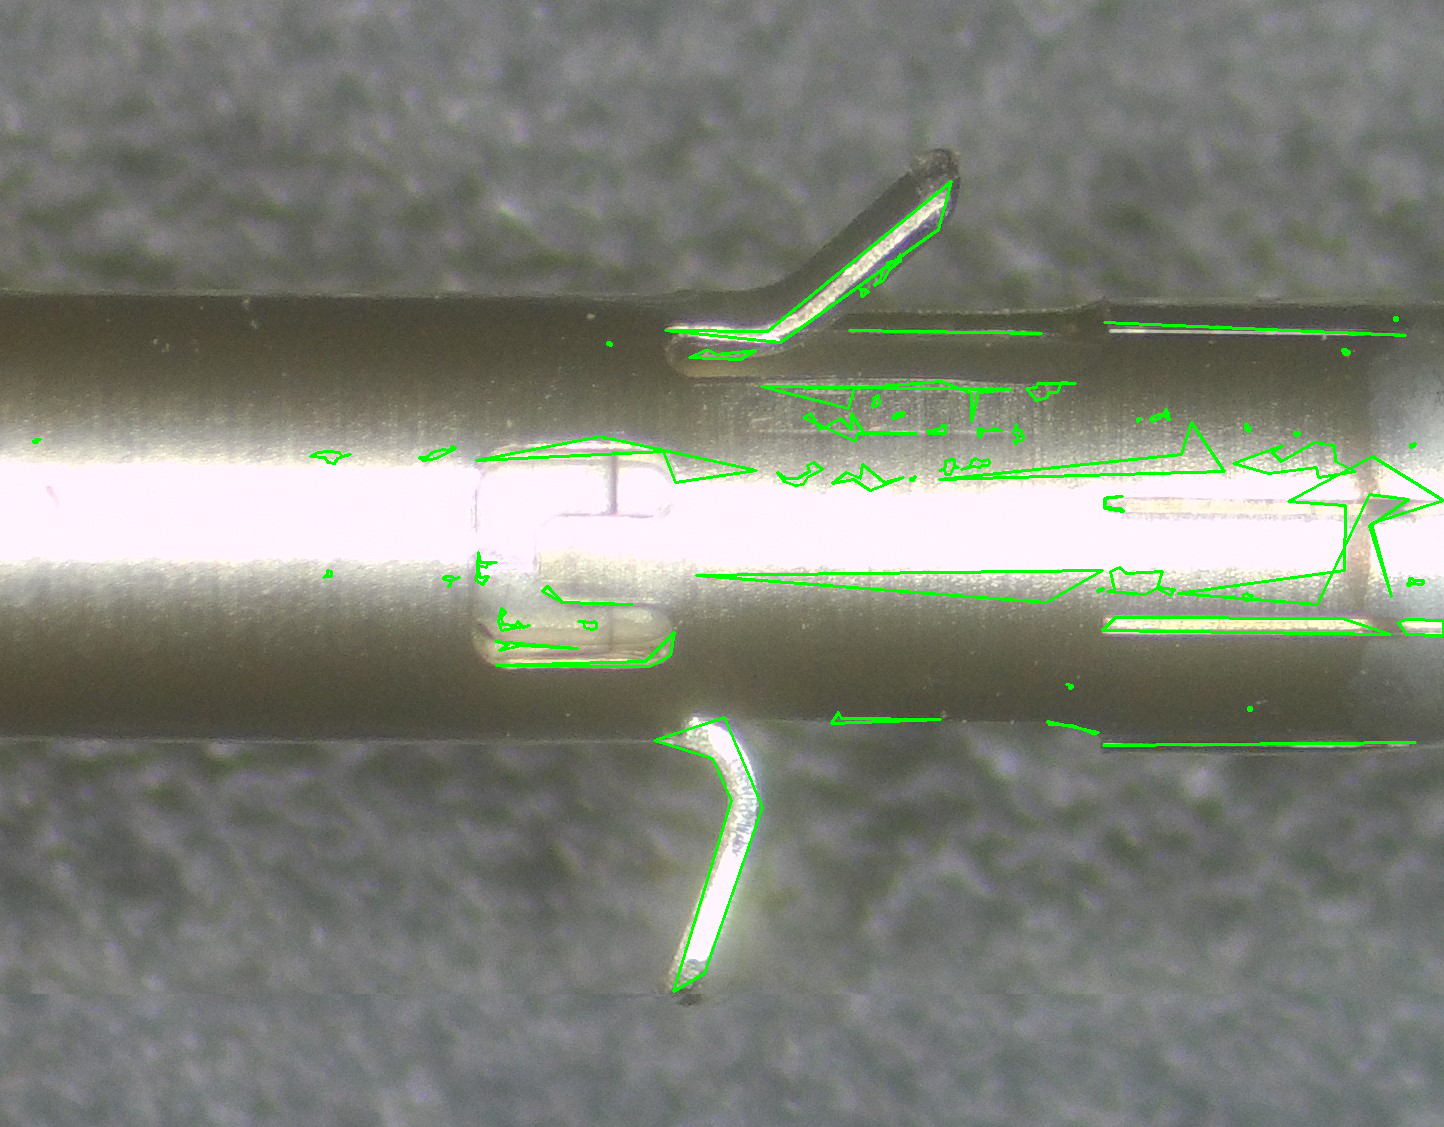
\includegraphics[width=\textwidth]{contours.png}
\captionof{figure}{Contours drew on image}
\end{center}
\end{enumerate}
\end{enumerate}
Due to the failure of finding contours of the whole object, I can not perform the remaining steps which I have proposed. The main reasons which lead to the failure are firstly, the background to likely salt-pepper noise with high ratio, secondly, the color the object is also like the color of the background, so that when applying Median filter or Gaussian filter then applying Canny edge detector, the result lost a lot of segmentations, and thirdly the angle of the light in the source input image is not optimal.\\
To improve the result, I would like to propose some ideas:
\begin{itemize}
\item Subtraction the background to extract only object
\item Take other input image with black or white color and better angle of light.
\end{itemize}
\pagebreak
\textbf{\large Reference}\\ \\
\big[1\big] http://is.hust.edu.vn/~oanhnt/GRK54/IPCV/\\ \\
\big[2\big] https://arxiv.org/abs/1512.03385\\ \\
\big[3\big] http://cs231n.stanford.edu/\\ \\
\big[4\big] https://www.pyimagesearch.com/opencv-tutorials-resources-guides/\\ \\

\end{document}
 to your LaTeX file where you want your
% title page.
%
%%%%%%%%%%%%%%%%%%%%%%%%%%%%%%%%%%%%%%%%%
%\title{bao cáo}
%----------------------------------------------------------------------------------------
%	PACKAGES AND OTHER DOCUMENT CONFIGURATIONS
%----------------------------------------------------------------------------------------

\documentclass[a4paper]{article}
\usepackage[english]{babel}
\usepackage[utf8x]{inputenc}
\usepackage{amsmath}
\usepackage{graphicx}
\usepackage[colorinlistoftodos]{todonotes}
\usepackage{listings}
\usepackage{color}
\usepackage{stackengine}
\usepackage{mathtools}
\usepackage{amsfonts}
\usepackage{wrapfig}
\usepackage{adjustbox}
\usepackage{gensymb}
\usepackage{hyperref}
\usepackage[font=small,labelfont=bf]{caption}
\usepackage[inline]{enumitem}
\definecolor{dkgreen}{rgb}{0,0.6,0}
\definecolor{gray}{rgb}{0.5,0.5,0.5}
\definecolor{mauve}{rgb}{0.58,0,0.82}

\lstset{
  language=C,
  aboveskip=3mm,
  belowskip=3mm,
  showstringspaces=false,
  columns=flexible,
  basicstyle={\small\ttfamily},
  numbers=none,
  numberstyle=\tiny\color{gray},
  keywordstyle=\color{blue},
  commentstyle=\color{dkgreen},
  stringstyle=\color{mauve},
  breaklines=true,
  breakatwhitespace=true,
  tabsize=3
}
\usepackage{titlesec}

\setcounter{secnumdepth}{4}

\titleformat{\paragraph}
{\normalfont\normalsize\bfseries}{\theparagraph}{1em}{}
\titlespacing*{\paragraph}
{0pt}{3.25ex plus 1ex minus .2ex}{1.5ex plus .2ex}
\newcommand*\conj[1]{\bar{#1}}
\newcommand*\mean[1]{\bar{#1}}
\begin{document}

\begin{titlepage}

\newcommand{\HRule}{\rule{\linewidth}{0.5mm}} % Defines a new command for the horizontal lines, change thickness here

\center % Center everything on the page
 
%----------------------------------------------------------------------------------------
%	HEADING SECTIONS
%----------------------------------------------------------------------------------------

\textsc{\Large Hanoi University of Science and Technology }\\[0.3cm] % Name of your university/college
\textsc{\large School of Information and Communication Technology}\\[3cm] % Major heading such as course name

\includegraphics[scale=0.4]{LogoBKchuan.jpg}\\[1cm] % Include a department/university logo - this will require the graphicx package
\textsc{\LARGE Graduation Research 1}\\
% \textsc{\Large Simple File Manager}\\[2cm]
 % Minor heading such as course title

% %----------------------------------------------------------------------------------------
% %	TITLE SECTION
% %----------------------------------------------------------------------------------------

\HRule \\[0.4cm]
{ \Large \bfseries Basic Image Principles, Operations and Neural Network in Computer Vision}\\[0.03cm] % Title of your document
\HRule \\[1.cm]

 
% %----------------------------------------------------------------------------------------
% %	AUTHOR SECTION
% %----------------------------------------------------------------------------------------

\begin{minipage}{1\textwidth}
\begin{flushleft} \large 
\emph{Student:}
Nguyen Dinh Hai Nam - 20143040 - ICT k59\\ % Your name

\end{flushleft}
\begin{flushleft} \large
\emph{Instructor:}
Ph.D Nguyen Thi Oanh
\end{flushleft}
\end{minipage}\\[2cm]

% If you don't want a supervisor, uncomment the two lines below and remove the section above
%\Large \emph{Author:}\\
%John \textsc{Smith}\\[3cm] % Your name

%------------------------------------------$----------------------------------------------
%	DATE SECTION
%----------------------------------------------------------------------------------------

{\large \today}\\[1cm] % Date, change the \today to a set date if you want to be precise



\vfill % Fill the rest of the page with whitespace

\end{titlepage}
\tableofcontents
\pagebreak

\section{Basic concepts:}
\subsection{Images}
\subsubsection{Definition:}
\begin{itemize}
\item An image is a 2D signal (x,y)
\item Mathematical point of view:
\begin{itemize}
\item An image is a matrix of numbers representing a signal.
\item Several tools exist to manipulate that signal.
\end{itemize}
\item Humanity point of view:
\begin{itemize}
\item An image contains many semantic information.
\item It needs to be interpreted beyond the value of numbers
\end{itemize}
\end{itemize}
\subsubsection{Classification:} There are 3 main types of images
\begin{itemize}
\item Gray level: representing images in black and white channels where distribution of  histogram in range $[0 ... 255]$
\item Binary images: each pixel of image has the value is $1$ or $0$
\item RGB images: representing images as a combination of 3 color channels Red-Green-Blue, distribution of histogram in each color channel in is in range $[0...255]$
\end{itemize}
\subsubsection{Properties:}
\begin{itemize}
\item Image sampling is limited by the capacity of the sensor, which is the number of pixels.
\item Image quantization: is limited by the quantity of tones defined for the interval.
\item Image representation: 
\begin{itemize}
\item Matrix of size $MxN$
\item Each value in the matrix is an integer values in range [0...255]
\end{itemize}
\item Image resolution:
\begin{itemize}
\item Spatial resolution: The smallest visible element.
\item Gray level resolution: The smallest visible color change.
\end{itemize}
\item Image luminance: is defined the mean of all gray levels in the image
\item Image contrast: is defined by standard deviation of the gray levels or the variation between the min and the max gray level
\end{itemize}
\subsection{Edge}
\subsubsection{Definition:}
An edge is a frontier(boder) separating two objects in an image.
\begin{itemize}
\item A discontinuity in the image.
\item Sometimes also referred as "\textit{contours}"
\end{itemize}
\subsubsection{Classifications:}
\begin{itemize}
\item 
\begin{minipage}[t]{\linewidth}
\raggedright Step edge: \hspace{3cm}
\adjustbox{valign=t}{%
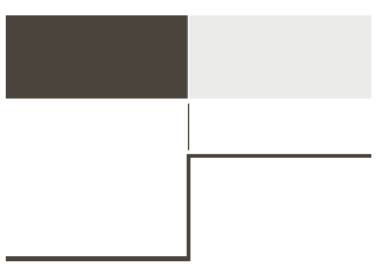
\includegraphics[width=.4\linewidth]{step-edge.png}%
}
\end{minipage}
\item 
\begin{minipage}[t]{\linewidth}
\raggedright Ramp edge: \hspace{3cm}
\adjustbox{valign=t}{%
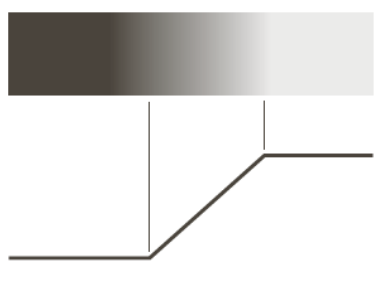
\includegraphics[width=.4\linewidth]{ramp-edge.png}%
}
\end{minipage}
\item 
\begin{minipage}[t]{\linewidth}
\raggedright Roof edge: \hspace{3cm}
\adjustbox{valign=t}{%
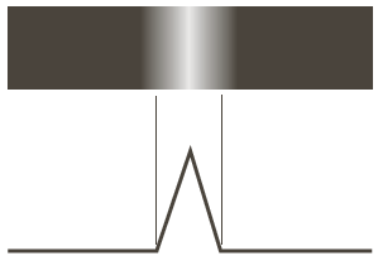
\includegraphics[width=.4\linewidth]{roof-edge.png}%
}
\end{minipage}
\end{itemize}
\pagebreak
Otherwise, edges can be affected by noise:
\begin{center}
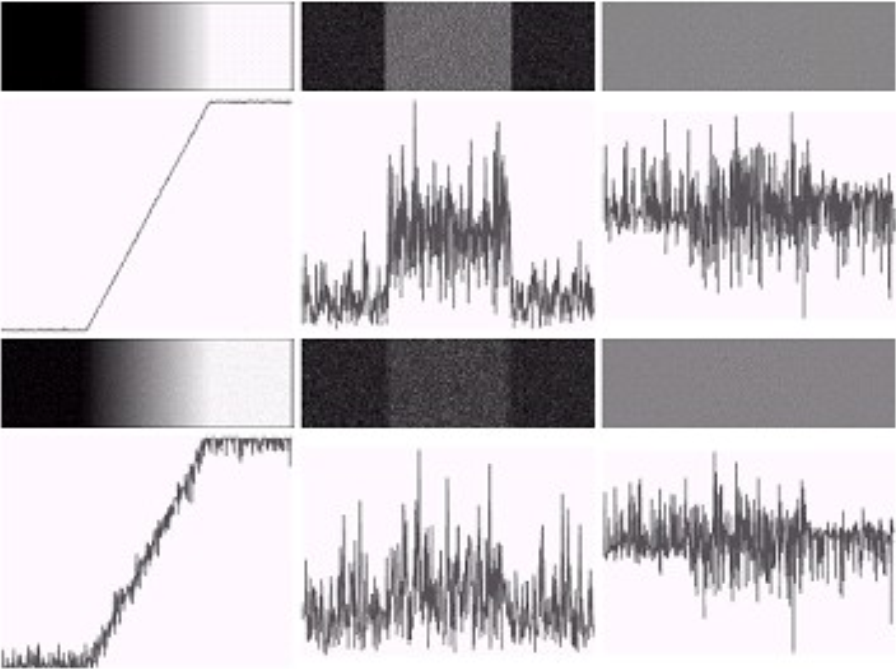
\includegraphics[width=\textwidth]{edge-noises.png}
\captionof{figure}{Edges with noise}
\end{center}
\subsubsection{Image derivative and edges:}
\subsubsection*{1.2.3.1 Image derivative:}
The first derivative ($gradient$) of the image is the base operator to measure edges in the image:
\begin{center}
$\mid \nabla f \mid \hspace{0.5cm} \equiv \Big( \frac{\partial f}{\partial x} \Big) ^2 \hspace{0.2cm} + \hspace{0.2cm} \Big(\frac{\partial f}{ \partial y}\Big)^2$
\end{center}
\begin{itemize}
\item 
\begin{minipage}[t]{\linewidth}
\raggedright Image histogram: \hspace{3cm}
\adjustbox{valign=t}{%
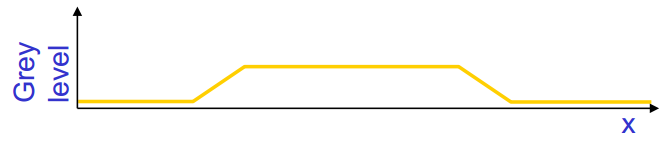
\includegraphics[width=.4\linewidth]{edge-histogram.png}%
}
\end{minipage}
\item 
\begin{minipage}[t]{\linewidth}
\raggedright First derivative $f'(x)$: \hspace{3cm}
\adjustbox{valign=t}{%
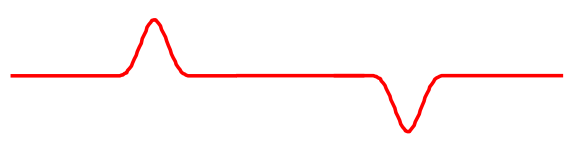
\includegraphics[width=.4\linewidth]{edge-1st-derivative.png}%
}
\end{minipage}
\item 
\begin{minipage}[t]{\linewidth}
\raggedright $\mid f'(x) \mid $  $\&$ threshold: \hspace{3cm}
\adjustbox{valign=t}{%
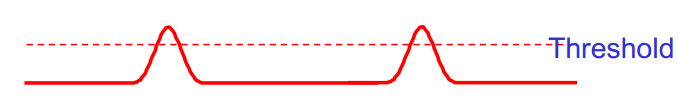
\includegraphics[width=.4\linewidth]{edge-2nd-derivative.png}%
}
\end{minipage}
\item 
\begin{minipage}[t]{\linewidth}
\raggedright $\mid f'(x) \mid $ $<$ threshold: \hspace{3cm}
\adjustbox{valign=t}{%
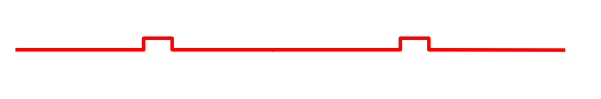
\includegraphics[width=.4\linewidth]{edge-filter.png}%
}
\end{minipage}
\end{itemize}
\pagebreak
\subsubsection{Filter/Kernel for detecting edges by convolution operation:}
\begin{itemize}
\item 
\begin{minipage}[t]{\linewidth}
\raggedright Roberts filter: \hspace{3cm}
\adjustbox{valign=t}{%
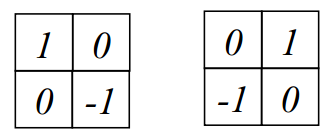
\includegraphics[width=.4\linewidth]{robert-filter.png}%
}
\end{minipage}
\item 
\begin{minipage}[t]{\linewidth}
\raggedright Sobel filter: \hspace{3cm}
\adjustbox{valign=t}{%
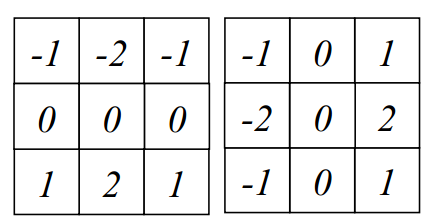
\includegraphics[width=.4\linewidth]{sobel-filter.png}%
}
\end{minipage}
\item 
\begin{minipage}[t]{\linewidth}
\raggedright Prewitt: \hspace{3cm}
\adjustbox{valign=t}{%
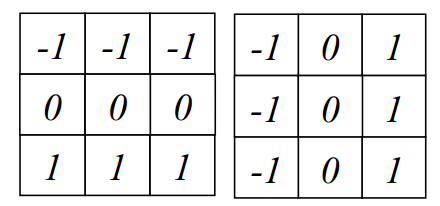
\includegraphics[width=.4\linewidth]{prewitt-filter.png}%
}
\end{minipage}
\end{itemize}
and etc...
\subsubsection{Image gradient:}
Derivative in X coordinate denoted as Gx, derivative in X coordinate denoted as Gy
\subsubsection*{1.2.5.1 Magnitude:}
Gradient intensity for each pixel:
\begin{center}
$
\mid G \mid \hspace{0.2cm} = \hspace{0.2cm} \sqrt{Gx^2 + Gy^2} \hspace{0.2cm} \approx \hspace{0.2cm} \mid Gx \mid \hspace{0.2cm} \mid Gy \mid 
$
\end{center}
\subsubsection*{1.2.5.2 Direction:}
Main gradient funtion for each pixel
\begin{center}
$
	\theta = arctan(Gy/Gx)
$
\end{center}
\subsubsection{Second image derivative}
Another approach to find edges in images is to use the \textit{second image derivative, for this, we use the $Laplacian$ as an operator}
\begin{center}
$
	\nabla ^ 2 I = \frac{\partial I}{\partial x ^2} + \frac{\partial I}{\partial y^2}
$
\end{center}
\subsubsection*{1.2.6.1 Laplacian using convolution:}
\begin{itemize}
\item Many discrete approximations exist for the Laplacian:
\[
  \begin{bmatrix}
    0 & 1 & 0\\
    1 & -4 & 1 \\
    0 & 1 & 0
  \end{bmatrix}
  \hspace{3cm}
    \begin{bmatrix}
    0 & 1 & 0\\
    1 & -8 & 1 \\
    0 & 1 & 0
  \end{bmatrix}
\]
\item One sole convolution matrix
\item Rotation symmetric
\end{itemize}
\subsubsection{Canny filter:}
Optimal filter for edge detection: filtering the image in several steps.\\ \par 
\subsubsection*{1.2.7.1.\hspace{0.5cm}Steps:}
\begin{enumerate}
\item Apply a Gaussian low-pass filter to remove noise on the image. 
\item Apply Sobel filter to the image and compute the gradient intensity and gradient direction in the image.
\item Non-maxima suppression: if the gradient magnitude of a pixel (x,y) is inferior to the one of its 2 neighbors along the gradient direction, then set this magnitude for (x,y) to zero.
\item Edge thressholding (hysteresis)
\begin{enumerate}
\item Use two thresholds: a threshold high (Sh) and a threshold low (Sb)
\item For each pixel in the gradient magnitude:
\begin{enumerate}
\item if $magnitude(x,y) < Sb$, then set this pixel to zero
\item If $magnitude(x,y) > Sh$, the set this pixel to edge pixel.
\item If $Sb < magnitude(x,y) \leq Sh$, then the pixel is set to edge pixel if it is connected to another edge pixel
\end{enumerate}
\end{enumerate}
\end{enumerate}
\subsection{Segmentation and Texture:}
\subsubsection{Segmentation:}
\subsubsection*{1.3.1.1\hspace{0.5cm}Definition:}
Segmentation aims to split an image into several parts which should correspond to object in the image
\subsubsection*{1.3.1.2\hspace{0.5cm} Goals:} 
Extract, separate elements in the image for applying a specific processing afterward or interpreting the image content.
\begin{itemize}
\item Discontinuities, edges: sudden changes, borders (frontier) between regions...
\item Homogeneous zones, regions: which has same colors, texture, intensity.
\end{itemize}
\subsubsection*{1.3.1.3\hspace{0.5cm}Methods:}
\begin{enumerate}
\item Thresholding
\begin{enumerate}
\item Histogram thresholding
\item Global thresholding
\item Multi-thresholding
\item Global automatic thresholding
\item Adaptive thresholding
\end{enumerate}
\item K-means algorithm
\item Split-and-merge
\item Watershed
\end{enumerate}
\subsubsection{Textures:}
\subsubsection*{1.3.2.1\hspace{0.5cm}Definition:}
Texture can be defined as a region with variation of intensity or as a spatial organization of pixels.
\subsubsection*{1.3.2.2\hspace{0.5cm}Methods:}
\begin{enumerate}
\item First order statistics: statistics on histogram
\item Co-occurence matrices: searching patterns
\item Frequential analysis: Gabor filter
\end{enumerate}
The most difficult is to find a good presentation for each texture.
\subsubsection{Color:}
\subsubsection*{1.3.3.1\hspace{0.5cm}Introduction:}
\begin{itemize}
\item Each pixel contains information from a spectral bandwidth.
\item We obtain color images, for example, by taking 3 bands from visible spectrum.
\item Some devices exist to acquire signal from more bands (X-ray, infrared, radio, ...)
\begin{center}
\includegraphics[width=\textwidth]{color-spectrum.png}
\captionof{figure}{Color spectrum}
\end{center}
\end{itemize}
\pagebreak
\subsubsection*{1.3.3.2\hspace{0.5cm}Primary colors:}
\begin{itemize}
\item RGB: Color representation using primary colors Red-Green-Blue:Additive scheme for displaying on a screen
\item CMY: Color representation using primary colors Cyan-Magenta-Yellow
\begin{itemize}
\item Subtractive scheme for printing on paper
\item We subtract from white instead of adding to black like in RGB
\item CMY = 1 - RGB
\end{itemize}
\end{itemize}
\begin{center}
\includegraphics[width=\textwidth]{rgbCMY.png}
\captionof{figure}{RGB - CMY color space}
\end{center}
\subsubsection*{1.3.3.3\hspace{0.5cm}Color spaces}
\begin{itemize}
\item There are many different spaces to represent colors.
\item RGB is the most common color representation in computer. 
\item There are three types of color spaces:
\begin{itemize}
\item Purely physic approach
\item Purely visual approach
\item Physic approach but corrected by psychometry
\end{itemize}
\end{itemize}
\subsubsection*{1.3.3.4\hspace{0.5cm}HSV representation:}
\begin{center}
\includegraphics[width=\textwidth]{hsv_colorspace.jpg}
\captionof{figure}{HSV color space}
\end{center}
\begin{itemize}
\item H-Hue is coded as an angle between 0 and 360$^{\circ}$
\item S-Saturation is coded as a radius between 0 and 1, S = 0 $\sim$ gray, S = 1 $\sim$ pure color
\item V-Value = MAX(Red, Green, Blue)
\end{itemize}
\section{Operations and Transformations:}
\subsection{Operations:}
\subsubsection{Contrast enhancement:}
\begin{itemize}
\item Linear Transformation: Enhance the dynamic range by linearly stretching the original gray levels to the range of target.
\item Piecewise Linear Transformation: Linear stretching with k segments.
\item Non-linear Transformation:
\begin{itemize}
\item Non-linear functions with a fixed form.
\item Fewer parameters to adjust.
\item Satisfying: $ 0 = f_{min} \leq g \leq f_{max} = L - 1$
\item Examples:
\begin{itemize}
\item Logarithmic transformation: stretch dark region, suppress bright region
\begin{center}
$ g = b.log(af +1) $
\end{center}
\item Exponential transformation: expand bright region
\begin{center}
$ g = b(e^{af} -1) $
\end{center}
\item Power law: $ g = af^k$\\
$k = 2$: square law, similar to exponential, $k = \frac{1}{3}$: cubic root, similar to logarithmic
\end{itemize}
\end{itemize}
\item Histogram Equalization:
Transform an image with arbitrary histogram to one with a flat histogram
\begin{itemize}
\item Suppose $f$ has PDF $p_F(f), 0 \leq f \leq 1$
\item Transform function (continuous): $g(f) = \int_{0}^{f}p_F(t)dt$
\end{itemize}
\end{itemize}
\subsubsection{Image operators}
\begin{itemize}
\item Logical operators: AND, OR, XOR, NOT 
\item Addition, Subtraction, Multiplication: add, subtract, multiply two pixels in two images with the corresponding position with upperbound 255 and lowerbound 0 into a new values of new image.
\end{itemize}
\subsubsection{Interpolation}
\begin{itemize}
\item Nearest Neighbor Interpolation:\\
Interpolation uses the values of the nearby translated pixel for the output pixel values.
\item Bilinear Interpolation:\\
The block uses the weighted average of two translated pixel values for each output pixel value.
\item Bicubic Interpolation:\\
The block uses the weighted average of four translated pixel values for each output pixel value.
\end{itemize}
\subsection{Transformations}
\subsubsection{Fourier Transforms:}
\begin{itemize}
\item Fourier transforms applied in Image Processing is Discrete Fourier Transforms because spatial domain from image is discrete
\item The output of the transformation represents the image in the frequency domain.
\begin{center}
$
	f(x,y) = \int_{-\infty}^{\infty}\int_{-\infty}^{\infty}F(u,v)e^{j2\pi (ux+uy)}dudv
$
\end{center}
\begin{center}
$
    F(u,v) = \int_{-\infty}^{\infty}\int_{-\infty}^{\infty}f(x,y)e^{j2\pi (ux+uy)}dxdy
$
\end{center}
where $u$ and $v$ are spatial frequencies
\item Fourier transformation produces a complex number valued output image. We use the real part to represent geometric structure of the spatial domain image. However, we need the real and the imaginary part to re-transform the image.
\begin{itemize}
\item $F(u,v)$ is complex in general
\begin{center}
$
	F(u,v) = F_R(u,v) + jF_i(u,v)
$
\end{center}
\item $\mid F(u,v)\mid$ is the magnitude spectrum
\item $\arctan(F_i(u,v)/F_R(u,v))$ is the phase angle spectrum
\end{itemize}
\item High frequencies: The points far from from FT center.
\item Low frequencies: The points near from FT center
\item Applications: Image analysis, image filtering, image reconstruction and image compression
\end{itemize}
\subsubsection{Hough transforms:}
\begin{itemize}
\item Hough transformation can be used to detect lines circles of used to detect other parametric curves.
\item It can give robust detection under noise and partial occlusion.
\item Transform line in $x-y$ space to point in $m-c$ space:
\begin{center}
\includegraphics[scale=0.4]{xy-mc.png}
\captionof{figure}{Line in xy space to point in mc space}
\end{center}
\item Transform point in $x-y$ space to line in $m-c$ space:
\begin{center}
\includegraphics[scale=0.4]{xy-mc-point.png}
\captionof{figure}{Point in xy space to line in mc space}
\end{center}
\item For Hough transform, taken an edge detected image, for every point that is non-black, draw lines in the $m-c$ space. Obviously, some lines will intersect. These intersections mark are the parameters of the line.
\begin{center}
\includegraphics[width=\textwidth]{xy-mc-example.png}
\captionof{figure}{Lines and points in xy space to points and lines in mc space}
\end{center}
\end{itemize}
\section{SIFT \& SURF:}
\subsection{SIFT}
\subsubsection{Description:}
The scale invariant feature transform, SIFT [17], extracts a set of descriptors from an image. The
extracted descriptors are invariant to image translation, rotation and scaling (zoom-out). SIFT
descriptors have also proved to be robust to a wide family of image transformations, such as slight
changes of viewpoint, noise, blur, contrast changes, scene deformation, while remaining discriminative
enough for matching purposes
\subsubsection{Algorithm:}
\begin{enumerate}
\item Compute the Gaussian scale-space defined as function $L(x,y,\sigma)$ with the variable-scale Gaussian $G(x,y,\sigma)$ and the input image $I(x,y)$: 
\begin{center}
$
	L(x,y,\sigma) = G(x,y,\sigma) * I(x,y)
$
\end{center}
where $*$ is convolution operation in x and y and $G(x,y,\sigma) = \frac{1}{2\pi \sigma^2}e^{-\frac{x^2+y^2}{2\sigma^2}} $
\item compute the Difference of Gaussians(DoG)
\begin{center}
$
	D(x,y,\sigma) = L(x,y,k\sigma) - L(x,y,\sigma)
$
\end{center}
\item Find candicate keypoints (3D discrete extrema of DoG) by comparing a pixel to its 26 neighbors in 3x3 regions at the current and adjacent scales.
\item Refine candicate keypoints location with sub-pixel precision.
\item Filter unstable keypoints due to noise.
\item Filter unstable keypoints lying on edge using Taylor expansion of scale-space function.
\item Assign a reference orientation to each keypoint based on scale-space gradient and orientation.
\item Build the keypoints d;escriptor ${(x,y,\sigma,\theta,\textbf{f})}$
\end{enumerate}
\subsection{SURF}
\subsubsection{Introduction:}
In computer vision, speeded up robust features (SURF) is a patented local feature detector and descriptor. It can be used for tasks such as object recognition, image registration, classification or 3D reconstruction. It is partly inspired by the scale-invariant feature transform (SIFT) descriptor
\subsubsection{Algorithm:}
To detect interest points, SURF uses an integer approximation of the determinant of Hessian blob detector, which can be computed with 3 integer operations using a precomputed integral image. Its feature descriptor is based on the sum of the Haar wavelet response around the point of interest. These can also be computed with the aid of the integral image.

SURF descriptors have been used to locate and recognize objects, people or faces, to reconstruct 3D scenes, to track objects and to extract points of interest.
\subsection{Comparison:}
\begin{enumerate}
\item Change of Viewpoint:
\begin{center}
\includegraphics[scale=0.3]{viewpoint.png}
\end{center}
\item Salt-pepper noise with rate of 0.5:
\begin{center}
\includegraphics[scale=0.3]{noisy.png}
\end{center}
\item Angle Variation of 45 $^{\circ}$:
\begin{center}
\includegraphics[scale=0.3]{angle-45.png}
\end{center}
\item Angle Variation of 90 $^{\circ}$:
\begin{center}
\includegraphics[scale=0.3]{angle-90.png}
\end{center}
\item Angle Variation of 135 $^{\circ}$:
\begin{center}
\includegraphics[scale=0.3]{angle-135.png}
\end{center}
\item Angle Variation of 180 $^{\circ}$:
\begin{center}
\includegraphics[scale=0.3]{angle-180.png}
\end{center}
\end{enumerate}



\section{Neural Network in Computer Vision:}
\subsection{Neural Network:}
\subsubsection{Definitions:}
An Artificial Neural Network is an information processing paradigm that is inspired by the way biological nervous system, such as brain, process information. The key element of this paradigm is the novel structure of the information processing system. It is composed of a large number of highly interconnected processing elements (neurones) working in unison to solve specific problems. ANNs, like people, learn by example. An ANN is configured for a specific application, such as pattern recognition or data classification, through a learning process. Learning in biological systems involves adjustments to the synaptic connections that exist between the neurones
\subsubsection{Architecture:}

Neural Network as neurons in graphs. Neural Networks are modeled as collections of neurons that are connected in an acyclic graph. In other words, the outputs of some neurons can become inputs to other neurons.
\begin{center}
\includegraphics[width=\textwidth]{nn-architecture.png}
\captionof{figure}{Neural Network with 2 hidden layers}
\end{center}
\begin{enumerate}
\item Input layer: this is the first layer of a neural network. It is used to provide the input data or features to the network
\item Output layer. Unlike all layers in a Neural Network, the output layer neurons most commonly do not have an activation function (or you can think of them as having a linear identity activation function). This is because the last output layer is usually taken to represent the class scores (e.g. in classification), which are arbitrary real-valued numbers, or some kind of real-valued target (e.g. in regression).
\item Hidden layer: A feedforward network applies a series of functions to the input. By having multiple hidden layers, we can compute complex functions by cascading simpler functions. The number of hidden layers is termed as the depth of the neural network. In general, deeper networks can learn more complex functions.
\end{enumerate}
\subsubsection{Activation Functions}
\begin{enumerate}
\item Sigmoid functions: It maps the input ($x$ axis) to values between 0 and 1.
\begin{center}
$
	\sigma(x) = \frac{1}{1+e^{-x}}
$
\end{center}
\begin{center}
\includegraphics[scale=0.5]{nn-sigmoid.png}
\captionof{figure}{sigmoid function}
\end{center}
In practice, the sigmoid non-linearity has recently fallen out of favor and it is rarely ever used. It has two major drawbacks:
\begin{itemize}
\item Sigmoid saturates and kills gradients: when the neuron’s activation saturates at either tail of 0 or 1, the gradient at these regions is almost zero. Therefore, if the local gradient is very small, it will effectively “kill” the gradient and almost no signal will flow through the neuron to its weights and recursively to its data.
\item Sigmoid outputs are not zero-centered:This has implications on the dynamics during gradient descent, because if the data coming into a neuron is always positive (e.g. $x>0$ elementwise in $f=wTx+b$)), then the gradient on the weights $w$ will during backpropagation become either all be positive, or all negative (depending on the gradient of the whole expression $f$). This could introduce undesirable zig-zagging dynamics in the gradient updates for the weights.
\end{itemize}
\item Tanh functions:It is similar to the sigmoid function butmaps the input to values between -1 and 1.
\begin{center}
$
	\tanh(x)=2\sigma(2x)−1 .
$
\end{center}
\begin{center}
\includegraphics[scale=0.5]{nn_tanh.png}
\captionof{figure}{tanh function}
\end{center}
Like the sigmoid neuron, its activations saturate, but unlike the sigmoid neuron its output is zero-centered. Therefore, in practice the tanh non-linearity is always preferred to the sigmoid nonlinearity.
\pagebreak
\item Rectified Linear Unit(ReLU): It allows only positive values to pass through it. The negative values are mapped to zero.
\begin{center}
$
	f(x)=\max(0,x)
$
\end{center}
\begin{center}
\includegraphics[scale=0.5]{nn-relu.png}
\captionof{figure}{ReLU function}
\end{center}
\begin{enumerate}
\item Advantages:
\begin{itemize}
\item It was found to greatly accelerate the convergence of stochastic gradient descent compared to the sigmoid/tanh functions.
\item  Compared to tanh/sigmoid neurons that involve expensive operations (exponentials, etc.), the ReLU can be implemented by simply thresholding a matrix of activations at zero.
\end{itemize}
\item Disadvantages:
\begin{itemize}
\item  ReLU units can be fragile during training and can “die”. For example, a large gradient flowing through a ReLU neuron could cause the weights to update in such a way that the neuron will never activate on any datapoint again. If this happens, then the gradient flowing through the unit will forever be zero from that point on
\end{itemize}
\end{enumerate}
\end{enumerate}
\pagebreak
\subsubsection{Optimization:}
\begin{center}
\includegraphics[width=\textwidth]{nn-optimization.png}
\captionof{figure}{Optimization}
\end{center}
The dataset of pairs of $(x,y)$ is given and fixed. The weights start out as random numbers and can change. During the forward pass the score function computes class scores, stored in vector $f$. The loss function contains two components: The data loss computes the compatibility between the scores $f$ and the labels $y$. The regularization loss is only a function of the weights. During Gradient Descent, we compute the gradient on the weights (and optionally on data if we wish) and use them to perform a parameter update during Gradient Descent.
\subsubsection{Backpropagation:}
A way of computing gradients of expressions through recursive application of chain rule.Our goal with backpropagation is to update each of the weights in the network so that they cause the actual output to be closer the target output, thereby minimizing the error for each output neuron and the network as a whole.
\subsection{Convolution Neural Network:}
\subsubsection{Definition:}
Convolutional Neural Networks are very similar to ordinary Neural Networks: they are made up of neurons that have learnable weights and biases. Each neuron receives some inputs, performs a dot product and optionally follows it with a non-linearity. The whole network still expresses a single differentiable score function: from the raw image pixels on one end to class scores at the other. And they still have a loss function (e.g. SVM/Softmax) on the last (fully-connected) layer and all the tips/tricks we developed for learning regular Neural Networks still apply
\subsubsection{Why Convolution Neural Network in Computer Vision:}
Input images for processing in Computer Vision usually consist of 3 channel colors with size MxN pixels, for example in CIFAR10 data set each image is size of 32x32x3 $\approx$ 3072 weights. Clearly, full connectivity in Regular Neural Nets  is wasteful and the huge number of parameters would quickly lead to overfitting and cause very costly computational. While Convolutional Neural Networks take advantage of the fact that the input consists of images and they constrain the architecture in a more sensible way. In particular, unlike a regular Neural Network, the layers of a ConvNet have neurons arranged in 3 dimensions: width, height, depth. The neurons in a layer will only be connected to a small region of the layer before it, instead of all of the neurons in a fully-connected manner
\subsubsection{Architecture:}
\begin{itemize}
\item CONV layer will compute the output of neurons that are connected to local regions in the input, each computing a dot product between their weights and a small region they are connected to in the input volume. 
\item RELU layer will apply an element-wise activation function, such as the max(0,x) thresholding at zero. 
\item POOL layer will perform a down-sampling operation along the spatial dimensions (width, height).
\item FC (i.e. fully-connected) layer will compute the class scores. As with ordinary Neural Networks and as the name implies, each neuron in this layer will be connected to all the numbers in the previous volume.
\end{itemize}
\section{Projects:}
\subsection{Environments, dataset, frameworks:}
\subsubsection{Environments:}
\begin{itemize}
\item OS: Linux - Ubuntu 16.04
\item Programing Language: Python (3.5) - an interpreted high-level programing language, close to human language.
\end{itemize}
\subsubsection{Dataset:}
\begin{itemize}
\item CIFAR10: a dataset consists of 60000 32x32 colour images in 10 classes, with 6000 images per class. There are 50000 training images and 10000 test images used for Classification.
\item Object images: high-resolution image of object to identify the error on it.
\end{itemize}
\subsubsection{Frameworks:}
\begin{itemize}
\item Anaconda: Free, open-source packages management and deployment aimed distribution of Python.
\item Scientific Python distributions: Numpy, Scipy, Matplotlib, ipython, jupyter, Pandas, SciKit learn.
\item Pytorch: a python package that provides two high-level features:
\begin{itemize}
\item Tensor computation (like Numpy) with strong GPU acceleration
\item Deep Neural Networks built on a tape-based autodiff system. 
\end{itemize}
\item OpenCV-Python: (Open Source Computer Vision Library) is an open source computer vision and machine learning software library. 
\end{itemize}
\subsection{Image Classification with CIFAR10 dataset:}
\subsubsection{Self-made convolution network:}
A simple Convolution Network with 3 CONV layers with MaxPooling layers, 3 FC layers and the the ReLu activation function was made to understand roles of each layer in CNN and how to implement a CNN in Pytorch.
\begin{itemize}
\item Models: \begin{itemize}
\item conv layer 1: $Conv2d(3, 12, kernel\_size=(5, 5), stride=(1, 1), padding=(2, 2))$
\item pool layer: $MaxPool2d(kernel\_size=2, stride=2, padding=0, dilation=1, ceil\_mode=False)$
\item conv layer 2: $Conv2d(12, 18, kernel\_size=(5, 5), stride=(1, 1), padding=(2, 2))$
\item pool layer: $MaxPool2d(kernel\_size=2, stride=2, padding=0, dilation=1, ceil\_mode=False)$
\item conv layer 3: $Conv2d(18, 26, kernel\_size=(3, 3), stride=(1, 1))$
\item pool layer: $MaxPool2d(kernel\_size=2, stride=2, padding=0, dilation=1, ceil\_mode=False)$
\item fc layer 1: $Linear(in\_features=234, out\_features=200, bias=True)$
\item fc layer 2: $Linear(in\_features=200, out\_features=84, bias=True)$
\item fc layer 3: $Linear(in\_features=84, out\_features=10, bias=True)$
\end{itemize}
With the ReLU activation function
\item Train loss: 1.547 and Accuracy: 45.96$\%$
\item Test loss: 1.335 and Accuracy: 54.740$\%$
\end{itemize}
\subsubsection{Residual Network (a.k.a ResNet):}
\subsubsection*{5.2.2.1\hspace{0.5cm}Why Residual Network?}
When Microsoft Research released Deep Residual Learning for Image Recognition in 2015, these networks led to 1st-place winning entries in all five main tracks of the ImageNet and COCO 2015 competitions, which covered image classification, object detection, and semantic segmentation. The robustness of ResNets has since been proven by various visual recognition tasks and by non-visual tasks involving speech and language.\\
\pagebreak
\par
Deep networks are hard to train because of the notorious vanishing or exploding gradient problem - as the gradient is back-propagated to earlier layers, repeated multiplication may make the gradient infinitively small. As a result, as the network goes deeper, its performance gets saturated or even starts degrading rapidly.
\begin{center}
\includegraphics[width=\textwidth]{train-test-error.png}
\captionof{figure}{Increasing network depth leads to worse performance}
\end{center}

\par The core idea of ResNet to tackle vanishing the above problems is introducing a so-called “identity shortcut connection” that skips one or more layers, as shown in the following figure:
\begin{center}
\includegraphics[width=\textwidth]{skip_connection.png}
\captionof{figure}{A residual block}
\end{center}
Skip connections which allows you to take the activation from one layer and suddenly feed it to another layer even much deeper in the neural network. And using that, ResNet enables to train very, very deep networks. \par
Instead of learning a direct mapping of $x->y$ with a function $H(x)$. Let define the residual function using $F(x) = H(x) - x$, which can be reframed into $H(x) = F(x)+x$, where $F(x)$ and $x$ represent the stacked non-linear layers and the identity function respectively. The author's hypothesis is that it is easy to optimize the residual mapping function $F(x)$ than to optimize the original, unreferenced mapping $H(x)$.
\pagebreak
\par The authors of [2] argue that stacking layers shouldn’t degrade the network performance, because we could simply stack identity mappings (layer that doesn’t do anything) upon the current network, and the resulting architecture would perform the same. This indicates that the deeper model should not produce a training error higher than its shallower counterparts. They hypothesize that letting the stacked layers fit a residual mapping is easier than letting them directly fit the desired underlaying mapping. And the residual block above explicitly allows it to do precisely that.
\begin{center}
\includegraphics[scale=0.3]{compare_resnet.png}
\captionof{figure}{ResNet Architecture}
\end{center}
\pagebreak
\par Furthermore, in ResNet, the authors proposed using Batch Normalization which also helps the network to solve vanishing gradients problem.
\begin{itemize}
\item Address the problem of vanishing/exploding gradients
\item Increase learning speed and solve many other problems
\item Each activation in every iteration each layer is normalized to have zero mean and variance 1 over a minibatch
\item Integrated into back-propagation algorithm
\end{itemize}
Batch Normalization:
\begin{itemize}
\item \textbf{Input:}Value of $x$ over a mini-batch $ B = \{ x_{1...m} \} $. Parameters to be learned: $\gamma, \beta$\\
\item \textbf{Output:}$ \{y_i = BN_{\gamma, \beta}(x_i)\}$
\begin{itemize}
\item Mini-batch mean:\hspace{0.2cm}$\mu_B \leftarrow \frac{1}{m}\Sigma^m_{i=1}x_i$\\[0.2cm]
\item Mini-batch variance:\hspace{0.2cm}$\sigma^2_B \leftarrow \frac{1}{m}\Sigma^m_{i=1}(x_i-\mu_B)^2 $\\[0.2cm]
\item Normalize:\hspace{0.2cm}$\hat{x_i} \leftarrow \frac{x_i - \mu_B}{\sqrt{\sigma^2_B + \epsilon}}$\\[0.2cm]
\item Scale and shift:\hspace{0.2cm}$y_i \leftarrow \gamma \hat{x_i} + \beta \equiv BN_{\gamma, \beta}(x_i) $
\end{itemize}
\end{itemize}
\subsubsection*{5.2.2.2\hspace{0.5cm}ResNet 34:}
To execute classification on CIFAR10 dataset, I would like to use ResNet 34 architecture in Residual Network framework. Due to availability on my own hardware to develop and debug and the experimental errors on the ImageNet data set.
\begin{center}
\includegraphics[scale=0.5]{image-net_err.png}
\captionof{figure}{Top-1 error($\%$, 10-crop testing)} on ImageNet validation.
\end{center}
\pagebreak
Intuitively, We have the architecture of the ResNets including ResNet 34.
\begin{center}
\includegraphics[width=\textwidth]{resnet-architecture.png}
\captionof{figure}{ResNets architecture}
\end{center}
\subsubsection*{5.2.2.3\hspace{0.5cm}Implementation and Results:}
\hspace{0.2cm} The code of this project has been public on Github: \\
\begin{center}
\url{https://github.com/t3min4l/pytorch-cifar10}
\end{center}
\par Result with 150 epochs, learning-rate: 0.1:\\ Best accuracy on Test set: 87.98\% while loss is 0.35
\subsubsection{Error detection on object in image:}
\subsubsection*{5.2.3.1\hspace{0.5cm}Propose idea:}
\begin{enumerate}
\item Find contour of the objects
\item Find minReact contain the contour
\item Find centroid of contour, and apply perspective transform
\item Draw midperpendiculars of the contour and split images in half
\item Detect differences by using function `compare$\_$ssim' from `skimage'
\end{enumerate}
\pagebreak
\subsubsection*{5.2.3.3\hspace{0.5cm}Execution:}
\begin{enumerate}
\item Find contour of the object:
\begin{enumerate}
\item Convert color from RGB to gray
\begin{center}
\includegraphics[width=\textwidth]{grayed.png}
\captionof{figure}{Convert image to gray scale}
\end{center}
\pagebreak
\item Apply Canny edge detector
\begin{center}
\includegraphics[width=\textwidth]{edged.png}
\captionof{figure}{Edges detected by Canny algorithm}
\end{center}
\pagebreak
\item Apply Morphological transformation
\begin{center}
\includegraphics[width=\textwidth]{mophor.png}
\captionof{figure}{Morphological gradients transformation}
\end{center}
\pagebreak
\item Find contours and draw them on the image
\begin{center}
\includegraphics[width=\textwidth]{contours.png}
\captionof{figure}{Contours drew on image}
\end{center}
\end{enumerate}
\end{enumerate}
Due to the failure of finding contours of the whole object, I can not perform the remaining steps which I have proposed. The main reasons which lead to the failure are firstly, the background to likely salt-pepper noise with high ratio, secondly, the color the object is also like the color of the background, so that when applying Median filter or Gaussian filter then applying Canny edge detector, the result lost a lot of segmentations, and thirdly the angle of the light in the source input image is not optimal.\\
To improve the result, I would like to propose some ideas:
\begin{itemize}
\item Subtraction the background to extract only object
\item Take other input image with black or white color and better angle of light.
\end{itemize}
\pagebreak
\textbf{\large Reference}\\ \\
\big[1\big] http://is.hust.edu.vn/~oanhnt/GRK54/IPCV/\\ \\
\big[2\big] https://arxiv.org/abs/1512.03385\\ \\
\big[3\big] http://cs231n.stanford.edu/\\ \\
\big[4\big] https://www.pyimagesearch.com/opencv-tutorials-resources-guides/\\ \\

\end{document}
 to your LaTeX file where you want your
% title page.
%
%%%%%%%%%%%%%%%%%%%%%%%%%%%%%%%%%%%%%%%%%
%\title{bao cáo}
%----------------------------------------------------------------------------------------
%	PACKAGES AND OTHER DOCUMENT CONFIGURATIONS
%----------------------------------------------------------------------------------------

\documentclass[a4paper]{article}
\usepackage[english]{babel}
\usepackage[utf8x]{inputenc}
\usepackage{amsmath}
\usepackage{graphicx}
\usepackage[colorinlistoftodos]{todonotes}
\usepackage{listings}
\usepackage{color}
\usepackage{stackengine}
\usepackage{mathtools}
\usepackage{amsfonts}
\usepackage{wrapfig}
\usepackage{adjustbox}
\usepackage{gensymb}
\usepackage{hyperref}
\usepackage[font=small,labelfont=bf]{caption}
\usepackage[inline]{enumitem}
\definecolor{dkgreen}{rgb}{0,0.6,0}
\definecolor{gray}{rgb}{0.5,0.5,0.5}
\definecolor{mauve}{rgb}{0.58,0,0.82}

\lstset{
  language=C,
  aboveskip=3mm,
  belowskip=3mm,
  showstringspaces=false,
  columns=flexible,
  basicstyle={\small\ttfamily},
  numbers=none,
  numberstyle=\tiny\color{gray},
  keywordstyle=\color{blue},
  commentstyle=\color{dkgreen},
  stringstyle=\color{mauve},
  breaklines=true,
  breakatwhitespace=true,
  tabsize=3
}
\usepackage{titlesec}

\setcounter{secnumdepth}{4}

\titleformat{\paragraph}
{\normalfont\normalsize\bfseries}{\theparagraph}{1em}{}
\titlespacing*{\paragraph}
{0pt}{3.25ex plus 1ex minus .2ex}{1.5ex plus .2ex}
\newcommand*\conj[1]{\bar{#1}}
\newcommand*\mean[1]{\bar{#1}}
\begin{document}

\begin{titlepage}

\newcommand{\HRule}{\rule{\linewidth}{0.5mm}} % Defines a new command for the horizontal lines, change thickness here

\center % Center everything on the page
 
%----------------------------------------------------------------------------------------
%	HEADING SECTIONS
%----------------------------------------------------------------------------------------

\textsc{\Large Hanoi University of Science and Technology }\\[0.3cm] % Name of your university/college
\textsc{\large School of Information and Communication Technology}\\[3cm] % Major heading such as course name
\includegraphics[scale=0.4]{LogoBKchuan.jpg}\\[1cm] % Include a department/university logo - this will require the graphicx package
\textsc{\LARGE Graduation Research 1}\\
% \textsc{\Large Simple File Manager}\\[2cm]
 % Minor heading such as course title

% %----------------------------------------------------------------------------------------
% %	TITLE SECTION
% %----------------------------------------------------------------------------------------

\HRule \\[0.4cm]
{ \Large \bfseries Basic Image Principles, Operations and Neural Network in Computer Vision}\\[0.03cm] % Title of your document
\HRule \\[1.cm]

 
% %----------------------------------------------------------------------------------------
% %	AUTHOR SECTION
% %----------------------------------------------------------------------------------------

\begin{minipage}{1\textwidth}
\begin{flushleft} \large 
\emph{Student:}
Nguyen Dinh Hai Nam - 20143040 - ICT k59\\ % Your name

\end{flushleft}
\begin{flushleft} \large
\emph{Instructor:}
Ph.D Nguyen Thi Oanh
\end{flushleft}
\end{minipage}\\[2cm]

% If you don't want a supervisor, uncomment the two lines below and remove the section above
%\Large \emph{Author:}\\
%John \textsc{Smith}\\[3cm] % Your name

%------------------------------------------$----------------------------------------------
%	DATE SECTION
%----------------------------------------------------------------------------------------

{\large \today}\\[1cm] % Date, change the \today to a set date if you want to be precise



\vfill % Fill the rest of the page with whitespace

\end{titlepage}
\tableofcontents
\pagebreak

\section{Basic concepts:}
\subsection{Images}
\subsubsection{Definition:}
\begin{itemize}
\item An image is a 2D signal (x,y)
\item Mathematical point of view:
\begin{itemize}
\item An image is a matrix of numbers representing a signal.
\item Several tools exist to manipulate that signal.
\end{itemize}
\item Humanity point of view:
\begin{itemize}
\item An image contains many semantic information.
\item It needs to be interpreted beyond the value of numbers
\end{itemize}
\end{itemize}
\subsubsection{Classification:} There are 3 main types of images
\begin{itemize}
\item Gray level: representing images in black and white channels where distribution of  histogram in range $[0 ... 255]$
\item Binary images: each pixel of image has the value is $1$ or $0$
\item RGB images: representing images as a combination of 3 color channels Red-Green-Blue, distribution of histogram in each color channel in is in range $[0...255]$
\end{itemize}
\subsubsection{Properties:}
\begin{itemize}
\item Image sampling is limited by the capacity of the sensor, which is the number of pixels.
\item Image quantization: is limited by the quantity of tones defined for the interval.
\item Image representation: 
\begin{itemize}
\item Matrix of size $MxN$
\item Each value in the matrix is an integer values in range [0...255]
\end{itemize}
\item Image resolution:
\begin{itemize}
\item Spatial resolution: The smallest visible element.
\item Gray level resolution: The smallest visible color change.
\end{itemize}
\item Image luminance: is defined the mean of all gray levels in the image
\item Image contrast: is defined by standard deviation of the gray levels or the variation between the min and the max gray level
\end{itemize}
\subsection{Edge}
\subsubsection{Definition:}
An edge is a frontier(boder) separating two objects in an image.
\begin{itemize}
\item A discontinuity in the image.
\item Sometimes also referred as "\textit{contours}"
\end{itemize}
\subsubsection{Classifications:}
\begin{itemize}
\item 
\begin{minipage}[t]{\linewidth}
\raggedright Step edge: \hspace{3cm}
\adjustbox{valign=t}{%
\includegraphics[width=.4\linewidth]{step-edge.png}%
}
\end{minipage}
\item 
\begin{minipage}[t]{\linewidth}
\raggedright Ramp edge: \hspace{3cm}
\adjustbox{valign=t}{%
\includegraphics[width=.4\linewidth]{ramp-edge.png}%
}
\end{minipage}
\item 
\begin{minipage}[t]{\linewidth}
\raggedright Roof edge: \hspace{3cm}
\adjustbox{valign=t}{%
\includegraphics[width=.4\linewidth]{roof-edge.png}%
}
\end{minipage}
\end{itemize}
\pagebreak
Otherwise, edges can be affected by noise:
\begin{center}
\includegraphics[width=\textwidth]{edge-noises.png}
\captionof{figure}{Edges with noise}
\end{center}
\subsubsection{Image derivative and edges:}
\subsubsection*{1.2.3.1 Image derivative:}
The first derivative ($gradient$) of the image is the base operator to measure edges in the image:
\begin{center}
$\mid \nabla f \mid \hspace{0.5cm} \equiv \Big( \frac{\partial f}{\partial x} \Big) ^2 \hspace{0.2cm} + \hspace{0.2cm} \Big(\frac{\partial f}{ \partial y}\Big)^2$
\end{center}
\begin{itemize}
\item 
\begin{minipage}[t]{\linewidth}
\raggedright Image histogram: \hspace{3cm}
\adjustbox{valign=t}{%
\includegraphics[width=.4\linewidth]{edge-histogram.png}%
}
\end{minipage}
\item 
\begin{minipage}[t]{\linewidth}
\raggedright First derivative $f'(x)$: \hspace{3cm}
\adjustbox{valign=t}{%
\includegraphics[width=.4\linewidth]{edge-1st-derivative.png}%
}
\end{minipage}
\item 
\begin{minipage}[t]{\linewidth}
\raggedright $\mid f'(x) \mid $  $\&$ threshold: \hspace{3cm}
\adjustbox{valign=t}{%
\includegraphics[width=.4\linewidth]{edge-2nd-derivative.png}%
}
\end{minipage}
\item 
\begin{minipage}[t]{\linewidth}
\raggedright $\mid f'(x) \mid $ $<$ threshold: \hspace{3cm}
\adjustbox{valign=t}{%
\includegraphics[width=.4\linewidth]{edge-filter.png}%
}
\end{minipage}
\end{itemize}
\pagebreak
\subsubsection{Filter/Kernel for detecting edges by convolution operation:}
\begin{itemize}
\item 
\begin{minipage}[t]{\linewidth}
\raggedright Roberts filter: \hspace{3cm}
\adjustbox{valign=t}{%
\includegraphics[width=.4\linewidth]{robert-filter.png}%
}
\end{minipage}
\item 
\begin{minipage}[t]{\linewidth}
\raggedright Sobel filter: \hspace{3cm}
\adjustbox{valign=t}{%
\includegraphics[width=.4\linewidth]{sobel-filter.png}%
}
\end{minipage}
\item 
\begin{minipage}[t]{\linewidth}
\raggedright Prewitt: \hspace{3cm}
\adjustbox{valign=t}{%
\includegraphics[width=.4\linewidth]{prewitt-filter.png}%
}
\end{minipage}
\end{itemize}
and etc...
\subsubsection{Image gradient:}
Derivative in X coordinate denoted as Gx, derivative in X coordinate denoted as Gy
\subsubsection*{1.2.5.1 Magnitude:}
Gradient intensity for each pixel:
\begin{center}
$
\mid G \mid \hspace{0.2cm} = \hspace{0.2cm} \sqrt{Gx^2 + Gy^2} \hspace{0.2cm} \approx \hspace{0.2cm} \mid Gx \mid \hspace{0.2cm} \mid Gy \mid 
$
\end{center}
\subsubsection*{1.2.5.2 Direction:}
Main gradient funtion for each pixel
\begin{center}
$
	\theta = arctan(Gy/Gx)
$
\end{center}
\subsubsection{Second image derivative}
Another approach to find edges in images is to use the \textit{second image derivative, for this, we use the $Laplacian$ as an operator}
\begin{center}
$
	\nabla ^ 2 I = \frac{\partial I}{\partial x ^2} + \frac{\partial I}{\partial y^2}
$
\end{center}
\subsubsection*{1.2.6.1 Laplacian using convolution:}
\begin{itemize}
\item Many discrete approximations exist for the Laplacian:
\[
  \begin{bmatrix}
    0 & 1 & 0\\
    1 & -4 & 1 \\
    0 & 1 & 0
  \end{bmatrix}
  \hspace{3cm}
    \begin{bmatrix}
    0 & 1 & 0\\
    1 & -8 & 1 \\
    0 & 1 & 0
  \end{bmatrix}
\]
\item One sole convolution matrix
\item Rotation symmetric
\end{itemize}
\subsubsection{Canny filter:}
Optimal filter for edge detection: filtering the image in several steps.\\ \par 
\subsubsection*{1.2.7.1.\hspace{0.5cm}Steps:}
\begin{enumerate}
\item Apply a Gaussian low-pass filter to remove noise on the image. 
\item Apply Sobel filter to the image and compute the gradient intensity and gradient direction in the image.
\item Non-maxima suppression: if the gradient magnitude of a pixel (x,y) is inferior to the one of its 2 neighbors along the gradient direction, then set this magnitude for (x,y) to zero.
\item Edge thressholding (hysteresis)
\begin{enumerate}
\item Use two thresholds: a threshold high (Sh) and a threshold low (Sb)
\item For each pixel in the gradient magnitude:
\begin{enumerate}
\item if $magnitude(x,y) < Sb$, then set this pixel to zero
\item If $magnitude(x,y) > Sh$, the set this pixel to edge pixel.
\item If $Sb < magnitude(x,y) \leq Sh$, then the pixel is set to edge pixel if it is connected to another edge pixel
\end{enumerate}
\end{enumerate}
\end{enumerate}
\subsection{Segmentation and Texture:}
\subsubsection{Segmentation:}
\subsubsection*{1.3.1.1\hspace{0.5cm}Definition:}
Segmentation aims to split an image into several parts which should correspond to object in the image
\subsubsection*{1.3.1.2\hspace{0.5cm} Goals:} 
Extract, separate elements in the image for applying a specific processing afterward or interpreting the image content.
\begin{itemize}
\item Discontinuities, edges: sudden changes, borders (frontier) between regions...
\item Homogeneous zones, regions: which has same colors, texture, intensity.
\end{itemize}
\subsubsection*{1.3.1.3\hspace{0.5cm}Methods:}
\begin{enumerate}
\item Thresholding
\begin{enumerate}
\item Histogram thresholding
\item Global thresholding
\item Multi-thresholding
\item Global automatic thresholding
\item Adaptive thresholding
\end{enumerate}
\item K-means algorithm
\item Split-and-merge
\item Watershed
\end{enumerate}
\subsubsection{Textures:}
\subsubsection*{1.3.2.1\hspace{0.5cm}Definition:}
Texture can be defined as a region with variation of intensity or as a spatial organization of pixels.
\subsubsection*{1.3.2.2\hspace{0.5cm}Methods:}
\begin{enumerate}
\item First order statistics: statistics on histogram
\item Co-occurence matrices: searching patterns
\item Frequential analysis: Gabor filter
\end{enumerate}
The most difficult is to find a good presentation for each texture.
\subsubsection{Color:}
\subsubsection*{1.3.3.1\hspace{0.5cm}Introduction:}
\begin{itemize}
\item Each pixel contains information from a spectral bandwidth.
\item We obtain color images, for example, by taking 3 bands from visible spectrum.
\item Some devices exist to acquire signal from more bands (X-ray, infrared, radio, ...)
\begin{center}
\includegraphics[width=\textwidth]{color-spectrum.png}
\captionof{figure}{Color spectrum}
\end{center}
\end{itemize}
\pagebreak
\subsubsection*{1.3.3.2\hspace{0.5cm}Primary colors:}
\begin{itemize}
\item RGB: Color representation using primary colors Red-Green-Blue:Additive scheme for displaying on a screen
\item CMY: Color representation using primary colors Cyan-Magenta-Yellow
\begin{itemize}
\item Subtractive scheme for printing on paper
\item We subtract from white instead of adding to black like in RGB
\item CMY = 1 - RGB
\end{itemize}
\end{itemize}
\begin{center}
\includegraphics[width=\textwidth]{rgbCMY.png}
\captionof{figure}{RGB - CMY color space}
\end{center}
\subsubsection*{1.3.3.3\hspace{0.5cm}Color spaces}
\begin{itemize}
\item There are many different spaces to represent colors.
\item RGB is the most common color representation in computer. 
\item There are three types of color spaces:
\begin{itemize}
\item Purely physic approach
\item Purely visual approach
\item Physic approach but corrected by psychometry
\end{itemize}
\end{itemize}
\subsubsection*{1.3.3.4\hspace{0.5cm}HSV representation:}
\begin{center}
\includegraphics[width=\textwidth]{hsv_colorspace.jpg}
\captionof{figure}{HSV color space}
\end{center}
\begin{itemize}
\item H-Hue is coded as an angle between 0 and 360$^{\circ}$
\item S-Saturation is coded as a radius between 0 and 1, S = 0 $\sim$ gray, S = 1 $\sim$ pure color
\item V-Value = MAX(Red, Green, Blue)
\end{itemize}
\section{Operations and Transformations:}
\subsection{Operations:}
\subsubsection{Contrast enhancement:}
\begin{itemize}
\item Linear Transformation: Enhance the dynamic range by linearly stretching the original gray levels to the range of target.
\item Piecewise Linear Transformation: Linear stretching with k segments.
\item Non-linear Transformation:
\begin{itemize}
\item Non-linear functions with a fixed form.
\item Fewer parameters to adjust.
\item Satisfying: $ 0 = f_{min} \leq g \leq f_{max} = L - 1$
\item Examples:
\begin{itemize}
\item Logarithmic transformation: stretch dark region, suppress bright region
\begin{center}
$ g = b.log(af +1) $
\end{center}
\item Exponential transformation: expand bright region
\begin{center}
$ g = b(e^{af} -1) $
\end{center}
\item Power law: $ g = af^k$\\
$k = 2$: square law, similar to exponential, $k = \frac{1}{3}$: cubic root, similar to logarithmic
\end{itemize}
\end{itemize}
\item Histogram Equalization:
Transform an image with arbitrary histogram to one with a flat histogram
\begin{itemize}
\item Suppose $f$ has PDF $p_F(f), 0 \leq f \leq 1$
\item Transform function (continuous): $g(f) = \int_{0}^{f}p_F(t)dt$
\end{itemize}
\end{itemize}
\subsubsection{Image operators}
\begin{itemize}
\item Logical operators: AND, OR, XOR, NOT 
\item Addition, Subtraction, Multiplication: add, subtract, multiply two pixels in two images with the corresponding position with upperbound 255 and lowerbound 0 into a new values of new image.
\end{itemize}
\subsubsection{Interpolation}
\begin{itemize}
\item Nearest Neighbor Interpolation:\\
Interpolation uses the values of the nearby translated pixel for the output pixel values.
\item Bilinear Interpolation:\\
The block uses the weighted average of two translated pixel values for each output pixel value.
\item Bicubic Interpolation:\\
The block uses the weighted average of four translated pixel values for each output pixel value.
\end{itemize}
\subsection{Transformations}
\subsubsection{Fourier Transforms:}
\begin{itemize}
\item Fourier transforms applied in Image Processing is Discrete Fourier Transforms because spatial domain from image is discrete
\item The output of the transformation represents the image in the frequency domain.
\begin{center}
$
	f(x,y) = \int_{-\infty}^{\infty}\int_{-\infty}^{\infty}F(u,v)e^{j2\pi (ux+uy)}dudv
$
\end{center}
\begin{center}
$
    F(u,v) = \int_{-\infty}^{\infty}\int_{-\infty}^{\infty}f(x,y)e^{j2\pi (ux+uy)}dxdy
$
\end{center}
where $u$ and $v$ are spatial frequencies
\item Fourier transformation produces a complex number valued output image. We use the real part to represent geometric structure of the spatial domain image. However, we need the real and the imaginary part to re-transform the image.
\begin{itemize}
\item $F(u,v)$ is complex in general
\begin{center}
$
	F(u,v) = F_R(u,v) + jF_i(u,v)
$
\end{center}
\item $\mid F(u,v)\mid$ is the magnitude spectrum
\item $\arctan(F_i(u,v)/F_R(u,v))$ is the phase angle spectrum
\end{itemize}
\item High frequencies: The points far from from FT center.
\item Low frequencies: The points near from FT center
\item Applications: Image analysis, image filtering, image reconstruction and image compression
\end{itemize}
\subsubsection{Hough transforms:}
\begin{itemize}
\item Hough transformation can be used to detect lines circles of used to detect other parametric curves.
\item It can give robust detection under noise and partial occlusion.
\item Transform line in $x-y$ space to point in $m-c$ space:
\begin{center}
\includegraphics[scale=0.4]{xy-mc.png}
\captionof{figure}{Line in xy space to point in mc space}
\end{center}
\item Transform point in $x-y$ space to line in $m-c$ space:
\begin{center}
\includegraphics[scale=0.4]{xy-mc-point.png}
\captionof{figure}{Point in xy space to line in mc space}
\end{center}
\item For Hough transform, taken an edge detected image, for every point that is non-black, draw lines in the $m-c$ space. Obviously, some lines will intersect. These intersections mark are the parameters of the line.
\begin{center}
\includegraphics[width=\textwidth]{xy-mc-example.png}
\captionof{figure}{Lines and points in xy space to points and lines in mc space}
\end{center}
\end{itemize}
\section{SIFT \& SURF:}
\subsection{SIFT}
\subsubsection{Description:}
The scale invariant feature transform, SIFT [17], extracts a set of descriptors from an image. The
extracted descriptors are invariant to image translation, rotation and scaling (zoom-out). SIFT
descriptors have also proved to be robust to a wide family of image transformations, such as slight
changes of viewpoint, noise, blur, contrast changes, scene deformation, while remaining discriminative
enough for matching purposes
\subsubsection{Algorithm:}
\begin{enumerate}
\item Compute the Gaussian scale-space defined as function $L(x,y,\sigma)$ with the variable-scale Gaussian $G(x,y,\sigma)$ and the input image $I(x,y)$: 
\begin{center}
$
	L(x,y,\sigma) = G(x,y,\sigma) * I(x,y)
$
\end{center}
where $*$ is convolution operation in x and y and $G(x,y,\sigma) = \frac{1}{2\pi \sigma^2}e^{-\frac{x^2+y^2}{2\sigma^2}} $
\item compute the Difference of Gaussians(DoG)
\begin{center}
$
	D(x,y,\sigma) = L(x,y,k\sigma) - L(x,y,\sigma)
$
\end{center}
\item Find candicate keypoints (3D discrete extrema of DoG) by comparing a pixel to its 26 neighbors in 3x3 regions at the current and adjacent scales.
\item Refine candicate keypoints location with sub-pixel precision.
\item Filter unstable keypoints due to noise.
\item Filter unstable keypoints lying on edge using Taylor expansion of scale-space function.
\item Assign a reference orientation to each keypoint based on scale-space gradient and orientation.
\item Build the keypoints d;escriptor ${(x,y,\sigma,\theta,\textbf{f})}$
\end{enumerate}
\subsection{SURF}
\subsubsection{Introduction:}
In computer vision, speeded up robust features (SURF) is a patented local feature detector and descriptor. It can be used for tasks such as object recognition, image registration, classification or 3D reconstruction. It is partly inspired by the scale-invariant feature transform (SIFT) descriptor
\subsubsection{Algorithm:}
To detect interest points, SURF uses an integer approximation of the determinant of Hessian blob detector, which can be computed with 3 integer operations using a precomputed integral image. Its feature descriptor is based on the sum of the Haar wavelet response around the point of interest. These can also be computed with the aid of the integral image.

SURF descriptors have been used to locate and recognize objects, people or faces, to reconstruct 3D scenes, to track objects and to extract points of interest.
\subsection{Comparison:}
\begin{enumerate}
\item Change of Viewpoint:
\begin{center}
\includegraphics[scale=0.3]{viewpoint.png}
\end{center}
\item Salt-pepper noise with rate of 0.5:
\begin{center}
\includegraphics[scale=0.3]{noisy.png}
\end{center}
\item Angle Variation of 45 $^{\circ}$:
\begin{center}
\includegraphics[scale=0.3]{angle-45.png}
\end{center}
\item Angle Variation of 90 $^{\circ}$:
\begin{center}
\includegraphics[scale=0.3]{angle-90.png}
\end{center}
\item Angle Variation of 135 $^{\circ}$:
\begin{center}
\includegraphics[scale=0.3]{angle-135.png}
\end{center}
\item Angle Variation of 180 $^{\circ}$:
\begin{center}
\includegraphics[scale=0.3]{angle-180.png}
\end{center}
\end{enumerate}



\section{Neural Network in Computer Vision:}
\subsection{Neural Network:}
\subsubsection{Definitions:}
An Artificial Neural Network is an information processing paradigm that is inspired by the way biological nervous system, such as brain, process information. The key element of this paradigm is the novel structure of the information processing system. It is composed of a large number of highly interconnected processing elements (neurones) working in unison to solve specific problems. ANNs, like people, learn by example. An ANN is configured for a specific application, such as pattern recognition or data classification, through a learning process. Learning in biological systems involves adjustments to the synaptic connections that exist between the neurones
\subsubsection{Architecture:}

Neural Network as neurons in graphs. Neural Networks are modeled as collections of neurons that are connected in an acyclic graph. In other words, the outputs of some neurons can become inputs to other neurons.
\begin{center}
\includegraphics[width=\textwidth]{nn-architecture.png}
\captionof{figure}{Neural Network with 2 hidden layers}
\end{center}
\begin{enumerate}
\item Input layer: this is the first layer of a neural network. It is used to provide the input data or features to the network
\item Output layer. Unlike all layers in a Neural Network, the output layer neurons most commonly do not have an activation function (or you can think of them as having a linear identity activation function). This is because the last output layer is usually taken to represent the class scores (e.g. in classification), which are arbitrary real-valued numbers, or some kind of real-valued target (e.g. in regression).
\item Hidden layer: A feedforward network applies a series of functions to the input. By having multiple hidden layers, we can compute complex functions by cascading simpler functions. The number of hidden layers is termed as the depth of the neural network. In general, deeper networks can learn more complex functions.
\end{enumerate}
\subsubsection{Activation Functions}
\begin{enumerate}
\item Sigmoid functions: It maps the input ($x$ axis) to values between 0 and 1.
\begin{center}
$
	\sigma(x) = \frac{1}{1+e^{-x}}
$
\end{center}
\begin{center}
\includegraphics[scale=0.5]{nn-sigmoid.png}
\captionof{figure}{sigmoid function}
\end{center}
In practice, the sigmoid non-linearity has recently fallen out of favor and it is rarely ever used. It has two major drawbacks:
\begin{itemize}
\item Sigmoid saturates and kills gradients: when the neuron’s activation saturates at either tail of 0 or 1, the gradient at these regions is almost zero. Therefore, if the local gradient is very small, it will effectively “kill” the gradient and almost no signal will flow through the neuron to its weights and recursively to its data.
\item Sigmoid outputs are not zero-centered:This has implications on the dynamics during gradient descent, because if the data coming into a neuron is always positive (e.g. $x>0$ elementwise in $f=wTx+b$)), then the gradient on the weights $w$ will during backpropagation become either all be positive, or all negative (depending on the gradient of the whole expression $f$). This could introduce undesirable zig-zagging dynamics in the gradient updates for the weights.
\end{itemize}
\item Tanh functions:It is similar to the sigmoid function butmaps the input to values between -1 and 1.
\begin{center}
$
	\tanh(x)=2\sigma(2x)−1 .
$
\end{center}
\begin{center}
\includegraphics[scale=0.5]{nn_tanh.png}
\captionof{figure}{tanh function}
\end{center}
Like the sigmoid neuron, its activations saturate, but unlike the sigmoid neuron its output is zero-centered. Therefore, in practice the tanh non-linearity is always preferred to the sigmoid nonlinearity.
\pagebreak
\item Rectified Linear Unit(ReLU): It allows only positive values to pass through it. The negative values are mapped to zero.
\begin{center}
$
	f(x)=\max(0,x)
$
\end{center}
\begin{center}
\includegraphics[scale=0.5]{nn-relu.png}
\captionof{figure}{ReLU function}
\end{center}
\begin{enumerate}
\item Advantages:
\begin{itemize}
\item It was found to greatly accelerate the convergence of stochastic gradient descent compared to the sigmoid/tanh functions.
\item  Compared to tanh/sigmoid neurons that involve expensive operations (exponentials, etc.), the ReLU can be implemented by simply thresholding a matrix of activations at zero.
\end{itemize}
\item Disadvantages:
\begin{itemize}
\item  ReLU units can be fragile during training and can “die”. For example, a large gradient flowing through a ReLU neuron could cause the weights to update in such a way that the neuron will never activate on any datapoint again. If this happens, then the gradient flowing through the unit will forever be zero from that point on
\end{itemize}
\end{enumerate}
\end{enumerate}
\pagebreak
\subsubsection{Optimization:}
\begin{center}
\includegraphics[width=\textwidth]{nn-optimization.png}
\captionof{figure}{Optimization}
\end{center}
The dataset of pairs of $(x,y)$ is given and fixed. The weights start out as random numbers and can change. During the forward pass the score function computes class scores, stored in vector $f$. The loss function contains two components: The data loss computes the compatibility between the scores $f$ and the labels $y$. The regularization loss is only a function of the weights. During Gradient Descent, we compute the gradient on the weights (and optionally on data if we wish) and use them to perform a parameter update during Gradient Descent.
\subsubsection{Backpropagation:}
A way of computing gradients of expressions through recursive application of chain rule.Our goal with backpropagation is to update each of the weights in the network so that they cause the actual output to be closer the target output, thereby minimizing the error for each output neuron and the network as a whole.
\subsection{Convolution Neural Network:}
\subsubsection{Definition:}
Convolutional Neural Networks are very similar to ordinary Neural Networks: they are made up of neurons that have learnable weights and biases. Each neuron receives some inputs, performs a dot product and optionally follows it with a non-linearity. The whole network still expresses a single differentiable score function: from the raw image pixels on one end to class scores at the other. And they still have a loss function (e.g. SVM/Softmax) on the last (fully-connected) layer and all the tips/tricks we developed for learning regular Neural Networks still apply
\subsubsection{Why Convolution Neural Network in Computer Vision:}
Input images for processing in Computer Vision usually consist of 3 channel colors with size MxN pixels, for example in CIFAR10 data set each image is size of 32x32x3 $\approx$ 3072 weights. Clearly, full connectivity in Regular Neural Nets  is wasteful and the huge number of parameters would quickly lead to overfitting and cause very costly computational. While Convolutional Neural Networks take advantage of the fact that the input consists of images and they constrain the architecture in a more sensible way. In particular, unlike a regular Neural Network, the layers of a ConvNet have neurons arranged in 3 dimensions: width, height, depth. The neurons in a layer will only be connected to a small region of the layer before it, instead of all of the neurons in a fully-connected manner
\subsubsection{Architecture:}
\begin{itemize}
\item CONV layer will compute the output of neurons that are connected to local regions in the input, each computing a dot product between their weights and a small region they are connected to in the input volume. 
\item RELU layer will apply an element-wise activation function, such as the max(0,x) thresholding at zero. 
\item POOL layer will perform a down-sampling operation along the spatial dimensions (width, height).
\item FC (i.e. fully-connected) layer will compute the class scores. As with ordinary Neural Networks and as the name implies, each neuron in this layer will be connected to all the numbers in the previous volume.
\end{itemize}
\section{Projects:}
\subsection{Environments, dataset, frameworks:}
\subsubsection{Environments:}
\begin{itemize}
\item OS: Linux - Ubuntu 16.04
\item Programing Language: Python (3.5) - an interpreted high-level programing language, close to human language.
\end{itemize}
\subsubsection{Dataset:}
\begin{itemize}
\item CIFAR10: a dataset consists of 60000 32x32 colour images in 10 classes, with 6000 images per class. There are 50000 training images and 10000 test images used for Classification.
\item Object images: high-resolution image of object to identify the error on it.
\end{itemize}
\subsubsection{Frameworks:}
\begin{itemize}
\item Anaconda: Free, open-source packages management and deployment aimed distribution of Python.
\item Scientific Python distributions: Numpy, Scipy, Matplotlib, ipython, jupyter, Pandas, SciKit learn.
\item Pytorch: a python package that provides two high-level features:
\begin{itemize}
\item Tensor computation (like Numpy) with strong GPU acceleration
\item Deep Neural Networks built on a tape-based autodiff system. 
\end{itemize}
\item OpenCV-Python: (Open Source Computer Vision Library) is an open source computer vision and machine learning software library. 
\end{itemize}
\subsection{Image Classification with CIFAR10 dataset:}
\subsubsection{Self-made convolution network:}
A simple Convolution Network with 3 CONV layers with MaxPooling layers, 3 FC layers and the the ReLu activation function was made to understand roles of each layer in CNN and how to implement a CNN in Pytorch.
\begin{itemize}
\item Models: \begin{itemize}
\item conv layer 1: $Conv2d(3, 12, kernel\_size=(5, 5), stride=(1, 1), padding=(2, 2))$
\item pool layer: $MaxPool2d(kernel\_size=2, stride=2, padding=0, dilation=1, ceil\_mode=False)$
\item conv layer 2: $Conv2d(12, 18, kernel\_size=(5, 5), stride=(1, 1), padding=(2, 2))$
\item pool layer: $MaxPool2d(kernel\_size=2, stride=2, padding=0, dilation=1, ceil\_mode=False)$
\item conv layer 3: $Conv2d(18, 26, kernel\_size=(3, 3), stride=(1, 1))$
\item pool layer: $MaxPool2d(kernel\_size=2, stride=2, padding=0, dilation=1, ceil\_mode=False)$
\item fc layer 1: $Linear(in\_features=234, out\_features=200, bias=True)$
\item fc layer 2: $Linear(in\_features=200, out\_features=84, bias=True)$
\item fc layer 3: $Linear(in\_features=84, out\_features=10, bias=True)$
\end{itemize}
With the ReLU activation function
\item Train loss: 1.547 and Accuracy: 45.96$\%$
\item Test loss: 1.335 and Accuracy: 54.740$\%$
\end{itemize}
\subsubsection{Residual Network (a.k.a ResNet):}
\subsubsection*{5.2.2.1\hspace{0.5cm}Why Residual Network?}
When Microsoft Research released Deep Residual Learning for Image Recognition in 2015, these networks led to 1st-place winning entries in all five main tracks of the ImageNet and COCO 2015 competitions, which covered image classification, object detection, and semantic segmentation. The robustness of ResNets has since been proven by various visual recognition tasks and by non-visual tasks involving speech and language.\\
\pagebreak
\par
Deep networks are hard to train because of the notorious vanishing or exploding gradient problem - as the gradient is back-propagated to earlier layers, repeated multiplication may make the gradient infinitively small. As a result, as the network goes deeper, its performance gets saturated or even starts degrading rapidly.
\begin{center}
\includegraphics[width=\textwidth]{train-test-error.png}
\captionof{figure}{Increasing network depth leads to worse performance}
\end{center}

\par The core idea of ResNet to tackle vanishing the above problems is introducing a so-called “identity shortcut connection” that skips one or more layers, as shown in the following figure:
\begin{center}
\includegraphics[width=\textwidth]{skip_connection.png}
\captionof{figure}{A residual block}
\end{center}
Skip connections which allows you to take the activation from one layer and suddenly feed it to another layer even much deeper in the neural network. And using that, ResNet enables to train very, very deep networks. \par
Instead of learning a direct mapping of $x->y$ with a function $H(x)$. Let define the residual function using $F(x) = H(x) - x$, which can be reframed into $H(x) = F(x)+x$, where $F(x)$ and $x$ represent the stacked non-linear layers and the identity function respectively. The author's hypothesis is that it is easy to optimize the residual mapping function $F(x)$ than to optimize the original, unreferenced mapping $H(x)$.
\pagebreak
\par The authors of [2] argue that stacking layers shouldn’t degrade the network performance, because we could simply stack identity mappings (layer that doesn’t do anything) upon the current network, and the resulting architecture would perform the same. This indicates that the deeper model should not produce a training error higher than its shallower counterparts. They hypothesize that letting the stacked layers fit a residual mapping is easier than letting them directly fit the desired underlaying mapping. And the residual block above explicitly allows it to do precisely that.
\begin{center}
\includegraphics[scale=0.3]{compare_resnet.png}
\captionof{figure}{ResNet Architecture}
\end{center}
\pagebreak
\par Furthermore, in ResNet, the authors proposed using Batch Normalization which also helps the network to solve vanishing gradients problem.
\begin{itemize}
\item Address the problem of vanishing/exploding gradients
\item Increase learning speed and solve many other problems
\item Each activation in every iteration each layer is normalized to have zero mean and variance 1 over a minibatch
\item Integrated into back-propagation algorithm
\end{itemize}
Batch Normalization:
\begin{itemize}
\item \textbf{Input:}Value of $x$ over a mini-batch $ B = \{ x_{1...m} \} $. Parameters to be learned: $\gamma, \beta$\\
\item \textbf{Output:}$ \{y_i = BN_{\gamma, \beta}(x_i)\}$
\begin{itemize}
\item Mini-batch mean:\hspace{0.2cm}$\mu_B \leftarrow \frac{1}{m}\Sigma^m_{i=1}x_i$\\[0.2cm]
\item Mini-batch variance:\hspace{0.2cm}$\sigma^2_B \leftarrow \frac{1}{m}\Sigma^m_{i=1}(x_i-\mu_B)^2 $\\[0.2cm]
\item Normalize:\hspace{0.2cm}$\hat{x_i} \leftarrow \frac{x_i - \mu_B}{\sqrt{\sigma^2_B + \epsilon}}$\\[0.2cm]
\item Scale and shift:\hspace{0.2cm}$y_i \leftarrow \gamma \hat{x_i} + \beta \equiv BN_{\gamma, \beta}(x_i) $
\end{itemize}
\end{itemize}
\subsubsection*{5.2.2.2\hspace{0.5cm}ResNet 34:}
To execute classification on CIFAR10 dataset, I would like to use ResNet 34 architecture in Residual Network framework. Due to availability on my own hardware to develop and debug and the experimental errors on the ImageNet data set.
\begin{center}
\includegraphics[scale=0.5]{image-net_err.png}
\captionof{figure}{Top-1 error($\%$, 10-crop testing)} on ImageNet validation.
\end{center}
\pagebreak
Intuitively, We have the architecture of the ResNets including ResNet 34.
\begin{center}
\includegraphics[width=\textwidth]{resnet-architecture.png}
\captionof{figure}{ResNets architecture}
\end{center}
\subsubsection*{5.2.2.3\hspace{0.5cm}Implementation and Results:}
\hspace{0.2cm} The code of this project has been public on Github: \\
\begin{center}
\url{https://github.com/t3min4l/pytorch-cifar10}
\end{center}
\par Result with 150 epochs, learning-rate: 0.1:\\ Best accuracy on Test set: 87.98\% while loss is 0.35
\subsubsection{Error detection on object in image:}
\subsubsection*{5.2.3.1\hspace{0.5cm}Propose idea:}
\begin{enumerate}
\item Find contour of the objects
\item Find minReact contain the contour
\item Find centroid of contour, and apply perspective transform
\item Draw midperpendiculars of the contour and split images in half
\item Detect differences by using function `compare$\_$ssim' from `skimage'
\end{enumerate}
\pagebreak
\subsubsection*{5.2.3.3\hspace{0.5cm}Execution:}
\begin{enumerate}
\item Find contour of the object:
\begin{enumerate}
\item Convert color from RGB to gray
\begin{center}
\includegraphics[width=\textwidth]{grayed.png}
\captionof{figure}{Convert image to gray scale}
\end{center}
\pagebreak
\item Apply Canny edge detector
\begin{center}
\includegraphics[width=\textwidth]{edged.png}
\captionof{figure}{Edges detected by Canny algorithm}
\end{center}
\pagebreak
\item Apply Morphological transformation
\begin{center}
\includegraphics[width=\textwidth]{mophor.png}
\captionof{figure}{Morphological gradients transformation}
\end{center}
\pagebreak
\item Find contours and draw them on the image
\begin{center}
\includegraphics[width=\textwidth]{contours.png}
\captionof{figure}{Contours drew on image}
\end{center}
\end{enumerate}
\end{enumerate}
Due to the failure of finding contours of the whole object, I can not perform the remaining steps which I have proposed. The main reasons which lead to the failure are firstly, the background to likely salt-pepper noise with high ratio, secondly, the color the object is also like the color of the background, so that when applying Median filter or Gaussian filter then applying Canny edge detector, the result lost a lot of segmentations, and thirdly the angle of the light in the source input image is not optimal.\\
To improve the result, I would like to propose some ideas:
\begin{itemize}
\item Subtraction the background to extract only object
\item Take other input image with black or white color and better angle of light.
\end{itemize}
\pagebreak
\textbf{\large Reference}\\ \\
\big[1\big] http://is.hust.edu.vn/~oanhnt/GRK54/IPCV/\\ \\
\big[2\big] https://arxiv.org/abs/1512.03385\\ \\
\big[3\big] http://cs231n.stanford.edu/\\ \\
\big[4\big] https://www.pyimagesearch.com/opencv-tutorials-resources-guides/\\ \\

\end{document}
 to your LaTeX file where you want your
% title page.
%
%%%%%%%%%%%%%%%%%%%%%%%%%%%%%%%%%%%%%%%%%
%\title{bao cáo}
%----------------------------------------------------------------------------------------
%	PACKAGES AND OTHER DOCUMENT CONFIGURATIONS
%----------------------------------------------------------------------------------------

\documentclass[a4paper]{article}
\usepackage[english]{babel}
\usepackage[utf8x]{inputenc}
\usepackage{amsmath}
\usepackage{graphicx}
\usepackage[colorinlistoftodos]{todonotes}
\usepackage{listings}
\usepackage{color}
\usepackage{stackengine}
\usepackage{mathtools}
\usepackage{amsfonts}
\usepackage{wrapfig}
\usepackage{adjustbox}
\usepackage{gensymb}
\usepackage{hyperref}
\usepackage[font=small,labelfont=bf]{caption}
\usepackage[inline]{enumitem}
\definecolor{dkgreen}{rgb}{0,0.6,0}
\definecolor{gray}{rgb}{0.5,0.5,0.5}
\definecolor{mauve}{rgb}{0.58,0,0.82}

\lstset{
  language=C,
  aboveskip=3mm,
  belowskip=3mm,
  showstringspaces=false,
  columns=flexible,
  basicstyle={\small\ttfamily},
  numbers=none,
  numberstyle=\tiny\color{gray},
  keywordstyle=\color{blue},
  commentstyle=\color{dkgreen},
  stringstyle=\color{mauve},
  breaklines=true,
  breakatwhitespace=true,
  tabsize=3
}
\usepackage{titlesec}

\setcounter{secnumdepth}{4}

\titleformat{\paragraph}
{\normalfont\normalsize\bfseries}{\theparagraph}{1em}{}
\titlespacing*{\paragraph}
{0pt}{3.25ex plus 1ex minus .2ex}{1.5ex plus .2ex}
\newcommand*\conj[1]{\bar{#1}}
\newcommand*\mean[1]{\bar{#1}}
\begin{document}

\begin{titlepage}

\newcommand{\HRule}{\rule{\linewidth}{0.5mm}} % Defines a new command for the horizontal lines, change thickness here

\center % Center everything on the page
 
%----------------------------------------------------------------------------------------
%	HEADING SECTIONS
%----------------------------------------------------------------------------------------

\textsc{\Large Hanoi University of Science and Technology }\\[0.3cm] % Name of your university/college
\textsc{\large School of Information and Communication Technology}\\[3cm] % Major heading such as course name
\includegraphics[scale=0.4]{LogoBKchuan.jpg}\\[1cm] % Include a department/university logo - this will require the graphicx package
\textsc{\LARGE Graduation Research 1}\\
% \textsc{\Large Simple File Manager}\\[2cm]
 % Minor heading such as course title

% %----------------------------------------------------------------------------------------
% %	TITLE SECTION
% %----------------------------------------------------------------------------------------

\HRule \\[0.4cm]
{ \Large \bfseries Basic Image Principles, Operations and Neural Network in Computer Vision}\\[0.03cm] % Title of your document
\HRule \\[1.cm]

 
% %----------------------------------------------------------------------------------------
% %	AUTHOR SECTION
% %----------------------------------------------------------------------------------------

\begin{minipage}{1\textwidth}
\begin{flushleft} \large 
\emph{Student:}
Nguyen Dinh Hai Nam - 20143040 - ICT k59\\ % Your name

\end{flushleft}
\begin{flushleft} \large
\emph{Instructor:}
Ph.D Nguyen Thi Oanh
\end{flushleft}
\end{minipage}\\[2cm]

% If you don't want a supervisor, uncomment the two lines below and remove the section above
%\Large \emph{Author:}\\
%John \textsc{Smith}\\[3cm] % Your name

%------------------------------------------$----------------------------------------------
%	DATE SECTION
%----------------------------------------------------------------------------------------

{\large \today}\\[1cm] % Date, change the \today to a set date if you want to be precise



\vfill % Fill the rest of the page with whitespace

\end{titlepage}
\tableofcontents
\pagebreak

\section{Basic concepts:}
\subsection{Images}
\subsubsection{Definition:}
\begin{itemize}
\item An image is a 2D signal (x,y)
\item Mathematical point of view:
\begin{itemize}
\item An image is a matrix of numbers representing a signal.
\item Several tools exist to manipulate that signal.
\end{itemize}
\item Humanity point of view:
\begin{itemize}
\item An image contains many semantic information.
\item It needs to be interpreted beyond the value of numbers
\end{itemize}
\end{itemize}
\subsubsection{Classification:} There are 3 main types of images
\begin{itemize}
\item Gray level: representing images in black and white channels where distribution of  histogram in range $[0 ... 255]$
\item Binary images: each pixel of image has the value is $1$ or $0$
\item RGB images: representing images as a combination of 3 color channels Red-Green-Blue, distribution of histogram in each color channel in is in range $[0...255]$
\end{itemize}
\subsubsection{Properties:}
\begin{itemize}
\item Image sampling is limited by the capacity of the sensor, which is the number of pixels.
\item Image quantization: is limited by the quantity of tones defined for the interval.
\item Image representation: 
\begin{itemize}
\item Matrix of size $MxN$
\item Each value in the matrix is an integer values in range [0...255]
\end{itemize}
\item Image resolution:
\begin{itemize}
\item Spatial resolution: The smallest visible element.
\item Gray level resolution: The smallest visible color change.
\end{itemize}
\item Image luminance: is defined the mean of all gray levels in the image
\item Image contrast: is defined by standard deviation of the gray levels or the variation between the min and the max gray level
\end{itemize}
\subsection{Edge}
\subsubsection{Definition:}
An edge is a frontier(boder) separating two objects in an image.
\begin{itemize}
\item A discontinuity in the image.
\item Sometimes also referred as "\textit{contours}"
\end{itemize}
\subsubsection{Classifications:}
\begin{itemize}
\item 
\begin{minipage}[t]{\linewidth}
\raggedright Step edge: \hspace{3cm}
\adjustbox{valign=t}{%
\includegraphics[width=.4\linewidth]{step-edge.png}%
}
\end{minipage}
\item 
\begin{minipage}[t]{\linewidth}
\raggedright Ramp edge: \hspace{3cm}
\adjustbox{valign=t}{%
\includegraphics[width=.4\linewidth]{ramp-edge.png}%
}
\end{minipage}
\item 
\begin{minipage}[t]{\linewidth}
\raggedright Roof edge: \hspace{3cm}
\adjustbox{valign=t}{%
\includegraphics[width=.4\linewidth]{roof-edge.png}%
}
\end{minipage}
\end{itemize}
\pagebreak
Otherwise, edges can be affected by noise:
\begin{center}
\includegraphics[width=\textwidth]{edge-noises.png}
\captionof{figure}{Edges with noise}
\end{center}
\subsubsection{Image derivative and edges:}
\subsubsection*{1.2.3.1 Image derivative:}
The first derivative ($gradient$) of the image is the base operator to measure edges in the image:
\begin{center}
$\mid \nabla f \mid \hspace{0.5cm} \equiv \Big( \frac{\partial f}{\partial x} \Big) ^2 \hspace{0.2cm} + \hspace{0.2cm} \Big(\frac{\partial f}{ \partial y}\Big)^2$
\end{center}
\begin{itemize}
\item 
\begin{minipage}[t]{\linewidth}
\raggedright Image histogram: \hspace{3cm}
\adjustbox{valign=t}{%
\includegraphics[width=.4\linewidth]{edge-histogram.png}%
}
\end{minipage}
\item 
\begin{minipage}[t]{\linewidth}
\raggedright First derivative $f'(x)$: \hspace{3cm}
\adjustbox{valign=t}{%
\includegraphics[width=.4\linewidth]{edge-1st-derivative.png}%
}
\end{minipage}
\item 
\begin{minipage}[t]{\linewidth}
\raggedright $\mid f'(x) \mid $  $\&$ threshold: \hspace{3cm}
\adjustbox{valign=t}{%
\includegraphics[width=.4\linewidth]{edge-2nd-derivative.png}%
}
\end{minipage}
\item 
\begin{minipage}[t]{\linewidth}
\raggedright $\mid f'(x) \mid $ $<$ threshold: \hspace{3cm}
\adjustbox{valign=t}{%
\includegraphics[width=.4\linewidth]{edge-filter.png}%
}
\end{minipage}
\end{itemize}
\pagebreak
\subsubsection{Filter/Kernel for detecting edges by convolution operation:}
\begin{itemize}
\item 
\begin{minipage}[t]{\linewidth}
\raggedright Roberts filter: \hspace{3cm}
\adjustbox{valign=t}{%
\includegraphics[width=.4\linewidth]{robert-filter.png}%
}
\end{minipage}
\item 
\begin{minipage}[t]{\linewidth}
\raggedright Sobel filter: \hspace{3cm}
\adjustbox{valign=t}{%
\includegraphics[width=.4\linewidth]{sobel-filter.png}%
}
\end{minipage}
\item 
\begin{minipage}[t]{\linewidth}
\raggedright Prewitt: \hspace{3cm}
\adjustbox{valign=t}{%
\includegraphics[width=.4\linewidth]{prewitt-filter.png}%
}
\end{minipage}
\end{itemize}
and etc...
\subsubsection{Image gradient:}
Derivative in X coordinate denoted as Gx, derivative in X coordinate denoted as Gy
\subsubsection*{1.2.5.1 Magnitude:}
Gradient intensity for each pixel:
\begin{center}
$
\mid G \mid \hspace{0.2cm} = \hspace{0.2cm} \sqrt{Gx^2 + Gy^2} \hspace{0.2cm} \approx \hspace{0.2cm} \mid Gx \mid \hspace{0.2cm} \mid Gy \mid 
$
\end{center}
\subsubsection*{1.2.5.2 Direction:}
Main gradient funtion for each pixel
\begin{center}
$
	\theta = arctan(Gy/Gx)
$
\end{center}
\subsubsection{Second image derivative}
Another approach to find edges in images is to use the \textit{second image derivative, for this, we use the $Laplacian$ as an operator}
\begin{center}
$
	\nabla ^ 2 I = \frac{\partial I}{\partial x ^2} + \frac{\partial I}{\partial y^2}
$
\end{center}
\subsubsection*{1.2.6.1 Laplacian using convolution:}
\begin{itemize}
\item Many discrete approximations exist for the Laplacian:
\[
  \begin{bmatrix}
    0 & 1 & 0\\
    1 & -4 & 1 \\
    0 & 1 & 0
  \end{bmatrix}
  \hspace{3cm}
    \begin{bmatrix}
    0 & 1 & 0\\
    1 & -8 & 1 \\
    0 & 1 & 0
  \end{bmatrix}
\]
\item One sole convolution matrix
\item Rotation symmetric
\end{itemize}
\subsubsection{Canny filter:}
Optimal filter for edge detection: filtering the image in several steps.\\ \par 
\subsubsection*{1.2.7.1.\hspace{0.5cm}Steps:}
\begin{enumerate}
\item Apply a Gaussian low-pass filter to remove noise on the image. 
\item Apply Sobel filter to the image and compute the gradient intensity and gradient direction in the image.
\item Non-maxima suppression: if the gradient magnitude of a pixel (x,y) is inferior to the one of its 2 neighbors along the gradient direction, then set this magnitude for (x,y) to zero.
\item Edge thressholding (hysteresis)
\begin{enumerate}
\item Use two thresholds: a threshold high (Sh) and a threshold low (Sb)
\item For each pixel in the gradient magnitude:
\begin{enumerate}
\item if $magnitude(x,y) < Sb$, then set this pixel to zero
\item If $magnitude(x,y) > Sh$, the set this pixel to edge pixel.
\item If $Sb < magnitude(x,y) \leq Sh$, then the pixel is set to edge pixel if it is connected to another edge pixel
\end{enumerate}
\end{enumerate}
\end{enumerate}
\subsection{Segmentation and Texture:}
\subsubsection{Segmentation:}
\subsubsection*{1.3.1.1\hspace{0.5cm}Definition:}
Segmentation aims to split an image into several parts which should correspond to object in the image
\subsubsection*{1.3.1.2\hspace{0.5cm} Goals:} 
Extract, separate elements in the image for applying a specific processing afterward or interpreting the image content.
\begin{itemize}
\item Discontinuities, edges: sudden changes, borders (frontier) between regions...
\item Homogeneous zones, regions: which has same colors, texture, intensity.
\end{itemize}
\subsubsection*{1.3.1.3\hspace{0.5cm}Methods:}
\begin{enumerate}
\item Thresholding
\begin{enumerate}
\item Histogram thresholding
\item Global thresholding
\item Multi-thresholding
\item Global automatic thresholding
\item Adaptive thresholding
\end{enumerate}
\item K-means algorithm
\item Split-and-merge
\item Watershed
\end{enumerate}
\subsubsection{Textures:}
\subsubsection*{1.3.2.1\hspace{0.5cm}Definition:}
Texture can be defined as a region with variation of intensity or as a spatial organization of pixels.
\subsubsection*{1.3.2.2\hspace{0.5cm}Methods:}
\begin{enumerate}
\item First order statistics: statistics on histogram
\item Co-occurence matrices: searching patterns
\item Frequential analysis: Gabor filter
\end{enumerate}
The most difficult is to find a good presentation for each texture.
\subsubsection{Color:}
\subsubsection*{1.3.3.1\hspace{0.5cm}Introduction:}
\begin{itemize}
\item Each pixel contains information from a spectral bandwidth.
\item We obtain color images, for example, by taking 3 bands from visible spectrum.
\item Some devices exist to acquire signal from more bands (X-ray, infrared, radio, ...)
\begin{center}
\includegraphics[width=\textwidth]{color-spectrum.png}
\captionof{figure}{Color spectrum}
\end{center}
\end{itemize}
\pagebreak
\subsubsection*{1.3.3.2\hspace{0.5cm}Primary colors:}
\begin{itemize}
\item RGB: Color representation using primary colors Red-Green-Blue:Additive scheme for displaying on a screen
\item CMY: Color representation using primary colors Cyan-Magenta-Yellow
\begin{itemize}
\item Subtractive scheme for printing on paper
\item We subtract from white instead of adding to black like in RGB
\item CMY = 1 - RGB
\end{itemize}
\end{itemize}
\begin{center}
\includegraphics[width=\textwidth]{rgbCMY.png}
\captionof{figure}{RGB - CMY color space}
\end{center}
\subsubsection*{1.3.3.3\hspace{0.5cm}Color spaces}
\begin{itemize}
\item There are many different spaces to represent colors.
\item RGB is the most common color representation in computer. 
\item There are three types of color spaces:
\begin{itemize}
\item Purely physic approach
\item Purely visual approach
\item Physic approach but corrected by psychometry
\end{itemize}
\end{itemize}
\subsubsection*{1.3.3.4\hspace{0.5cm}HSV representation:}
\begin{center}
\includegraphics[width=\textwidth]{hsv_colorspace.jpg}
\captionof{figure}{HSV color space}
\end{center}
\begin{itemize}
\item H-Hue is coded as an angle between 0 and 360$^{\circ}$
\item S-Saturation is coded as a radius between 0 and 1, S = 0 $\sim$ gray, S = 1 $\sim$ pure color
\item V-Value = MAX(Red, Green, Blue)
\end{itemize}
\section{Operations and Transformations:}
\subsection{Operations:}
\subsubsection{Contrast enhancement:}
\begin{itemize}
\item Linear Transformation: Enhance the dynamic range by linearly stretching the original gray levels to the range of target.
\item Piecewise Linear Transformation: Linear stretching with k segments.
\item Non-linear Transformation:
\begin{itemize}
\item Non-linear functions with a fixed form.
\item Fewer parameters to adjust.
\item Satisfying: $ 0 = f_{min} \leq g \leq f_{max} = L - 1$
\item Examples:
\begin{itemize}
\item Logarithmic transformation: stretch dark region, suppress bright region
\begin{center}
$ g = b.log(af +1) $
\end{center}
\item Exponential transformation: expand bright region
\begin{center}
$ g = b(e^{af} -1) $
\end{center}
\item Power law: $ g = af^k$\\
$k = 2$: square law, similar to exponential, $k = \frac{1}{3}$: cubic root, similar to logarithmic
\end{itemize}
\end{itemize}
\item Histogram Equalization:
Transform an image with arbitrary histogram to one with a flat histogram
\begin{itemize}
\item Suppose $f$ has PDF $p_F(f), 0 \leq f \leq 1$
\item Transform function (continuous): $g(f) = \int_{0}^{f}p_F(t)dt$
\end{itemize}
\end{itemize}
\subsubsection{Image operators}
\begin{itemize}
\item Logical operators: AND, OR, XOR, NOT 
\item Addition, Subtraction, Multiplication: add, subtract, multiply two pixels in two images with the corresponding position with upperbound 255 and lowerbound 0 into a new values of new image.
\end{itemize}
\subsubsection{Interpolation}
\begin{itemize}
\item Nearest Neighbor Interpolation:\\
Interpolation uses the values of the nearby translated pixel for the output pixel values.
\item Bilinear Interpolation:\\
The block uses the weighted average of two translated pixel values for each output pixel value.
\item Bicubic Interpolation:\\
The block uses the weighted average of four translated pixel values for each output pixel value.
\end{itemize}
\subsection{Transformations}
\subsubsection{Fourier Transforms:}
\begin{itemize}
\item Fourier transforms applied in Image Processing is Discrete Fourier Transforms because spatial domain from image is discrete
\item The output of the transformation represents the image in the frequency domain.
\begin{center}
$
	f(x,y) = \int_{-\infty}^{\infty}\int_{-\infty}^{\infty}F(u,v)e^{j2\pi (ux+uy)}dudv
$
\end{center}
\begin{center}
$
    F(u,v) = \int_{-\infty}^{\infty}\int_{-\infty}^{\infty}f(x,y)e^{j2\pi (ux+uy)}dxdy
$
\end{center}
where $u$ and $v$ are spatial frequencies
\item Fourier transformation produces a complex number valued output image. We use the real part to represent geometric structure of the spatial domain image. However, we need the real and the imaginary part to re-transform the image.
\begin{itemize}
\item $F(u,v)$ is complex in general
\begin{center}
$
	F(u,v) = F_R(u,v) + jF_i(u,v)
$
\end{center}
\item $\mid F(u,v)\mid$ is the magnitude spectrum
\item $\arctan(F_i(u,v)/F_R(u,v))$ is the phase angle spectrum
\end{itemize}
\item High frequencies: The points far from from FT center.
\item Low frequencies: The points near from FT center
\item Applications: Image analysis, image filtering, image reconstruction and image compression
\end{itemize}
\subsubsection{Hough transforms:}
\begin{itemize}
\item Hough transformation can be used to detect lines circles of used to detect other parametric curves.
\item It can give robust detection under noise and partial occlusion.
\item Transform line in $x-y$ space to point in $m-c$ space:
\begin{center}
\includegraphics[scale=0.4]{xy-mc.png}
\captionof{figure}{Line in xy space to point in mc space}
\end{center}
\item Transform point in $x-y$ space to line in $m-c$ space:
\begin{center}
\includegraphics[scale=0.4]{xy-mc-point.png}
\captionof{figure}{Point in xy space to line in mc space}
\end{center}
\item For Hough transform, taken an edge detected image, for every point that is non-black, draw lines in the $m-c$ space. Obviously, some lines will intersect. These intersections mark are the parameters of the line.
\begin{center}
\includegraphics[width=\textwidth]{xy-mc-example.png}
\captionof{figure}{Lines and points in xy space to points and lines in mc space}
\end{center}
\end{itemize}
\section{SIFT \& SURF:}
\subsection{SIFT}
\subsubsection{Description:}
The scale invariant feature transform, SIFT [17], extracts a set of descriptors from an image. The
extracted descriptors are invariant to image translation, rotation and scaling (zoom-out). SIFT
descriptors have also proved to be robust to a wide family of image transformations, such as slight
changes of viewpoint, noise, blur, contrast changes, scene deformation, while remaining discriminative
enough for matching purposes
\subsubsection{Algorithm:}
\begin{enumerate}
\item Compute the Gaussian scale-space defined as function $L(x,y,\sigma)$ with the variable-scale Gaussian $G(x,y,\sigma)$ and the input image $I(x,y)$: 
\begin{center}
$
	L(x,y,\sigma) = G(x,y,\sigma) * I(x,y)
$
\end{center}
where $*$ is convolution operation in x and y and $G(x,y,\sigma) = \frac{1}{2\pi \sigma^2}e^{-\frac{x^2+y^2}{2\sigma^2}} $
\item compute the Difference of Gaussians(DoG)
\begin{center}
$
	D(x,y,\sigma) = L(x,y,k\sigma) - L(x,y,\sigma)
$
\end{center}
\item Find candicate keypoints (3D discrete extrema of DoG) by comparing a pixel to its 26 neighbors in 3x3 regions at the current and adjacent scales.
\item Refine candicate keypoints location with sub-pixel precision.
\item Filter unstable keypoints due to noise.
\item Filter unstable keypoints lying on edge using Taylor expansion of scale-space function.
\item Assign a reference orientation to each keypoint based on scale-space gradient and orientation.
\item Build the keypoints d;escriptor ${(x,y,\sigma,\theta,\textbf{f})}$
\end{enumerate}
\subsection{SURF}
\subsubsection{Introduction:}
In computer vision, speeded up robust features (SURF) is a patented local feature detector and descriptor. It can be used for tasks such as object recognition, image registration, classification or 3D reconstruction. It is partly inspired by the scale-invariant feature transform (SIFT) descriptor
\subsubsection{Algorithm:}
To detect interest points, SURF uses an integer approximation of the determinant of Hessian blob detector, which can be computed with 3 integer operations using a precomputed integral image. Its feature descriptor is based on the sum of the Haar wavelet response around the point of interest. These can also be computed with the aid of the integral image.

SURF descriptors have been used to locate and recognize objects, people or faces, to reconstruct 3D scenes, to track objects and to extract points of interest.
\subsection{Comparison:}
\begin{enumerate}
\item Change of Viewpoint:
\begin{center}
\includegraphics[scale=0.3]{viewpoint.png}
\end{center}
\item Salt-pepper noise with rate of 0.5:
\begin{center}
\includegraphics[scale=0.3]{noisy.png}
\end{center}
\item Angle Variation of 45 $^{\circ}$:
\begin{center}
\includegraphics[scale=0.3]{angle-45.png}
\end{center}
\item Angle Variation of 90 $^{\circ}$:
\begin{center}
\includegraphics[scale=0.3]{angle-90.png}
\end{center}
\item Angle Variation of 135 $^{\circ}$:
\begin{center}
\includegraphics[scale=0.3]{angle-135.png}
\end{center}
\item Angle Variation of 180 $^{\circ}$:
\begin{center}
\includegraphics[scale=0.3]{angle-180.png}
\end{center}
\end{enumerate}



\section{Neural Network in Computer Vision:}
\subsection{Neural Network:}
\subsubsection{Definitions:}
An Artificial Neural Network is an information processing paradigm that is inspired by the way biological nervous system, such as brain, process information. The key element of this paradigm is the novel structure of the information processing system. It is composed of a large number of highly interconnected processing elements (neurones) working in unison to solve specific problems. ANNs, like people, learn by example. An ANN is configured for a specific application, such as pattern recognition or data classification, through a learning process. Learning in biological systems involves adjustments to the synaptic connections that exist between the neurones
\subsubsection{Architecture:}

Neural Network as neurons in graphs. Neural Networks are modeled as collections of neurons that are connected in an acyclic graph. In other words, the outputs of some neurons can become inputs to other neurons.
\begin{center}
\includegraphics[width=\textwidth]{nn-architecture.png}
\captionof{figure}{Neural Network with 2 hidden layers}
\end{center}
\begin{enumerate}
\item Input layer: this is the first layer of a neural network. It is used to provide the input data or features to the network
\item Output layer. Unlike all layers in a Neural Network, the output layer neurons most commonly do not have an activation function (or you can think of them as having a linear identity activation function). This is because the last output layer is usually taken to represent the class scores (e.g. in classification), which are arbitrary real-valued numbers, or some kind of real-valued target (e.g. in regression).
\item Hidden layer: A feedforward network applies a series of functions to the input. By having multiple hidden layers, we can compute complex functions by cascading simpler functions. The number of hidden layers is termed as the depth of the neural network. In general, deeper networks can learn more complex functions.
\end{enumerate}
\subsubsection{Activation Functions}
\begin{enumerate}
\item Sigmoid functions: It maps the input ($x$ axis) to values between 0 and 1.
\begin{center}
$
	\sigma(x) = \frac{1}{1+e^{-x}}
$
\end{center}
\begin{center}
\includegraphics[scale=0.5]{nn-sigmoid.png}
\captionof{figure}{sigmoid function}
\end{center}
In practice, the sigmoid non-linearity has recently fallen out of favor and it is rarely ever used. It has two major drawbacks:
\begin{itemize}
\item Sigmoid saturates and kills gradients: when the neuron’s activation saturates at either tail of 0 or 1, the gradient at these regions is almost zero. Therefore, if the local gradient is very small, it will effectively “kill” the gradient and almost no signal will flow through the neuron to its weights and recursively to its data.
\item Sigmoid outputs are not zero-centered:This has implications on the dynamics during gradient descent, because if the data coming into a neuron is always positive (e.g. $x>0$ elementwise in $f=wTx+b$)), then the gradient on the weights $w$ will during backpropagation become either all be positive, or all negative (depending on the gradient of the whole expression $f$). This could introduce undesirable zig-zagging dynamics in the gradient updates for the weights.
\end{itemize}
\item Tanh functions:It is similar to the sigmoid function butmaps the input to values between -1 and 1.
\begin{center}
$
	\tanh(x)=2\sigma(2x)−1 .
$
\end{center}
\begin{center}
\includegraphics[scale=0.5]{nn_tanh.png}
\captionof{figure}{tanh function}
\end{center}
Like the sigmoid neuron, its activations saturate, but unlike the sigmoid neuron its output is zero-centered. Therefore, in practice the tanh non-linearity is always preferred to the sigmoid nonlinearity.
\pagebreak
\item Rectified Linear Unit(ReLU): It allows only positive values to pass through it. The negative values are mapped to zero.
\begin{center}
$
	f(x)=\max(0,x)
$
\end{center}
\begin{center}
\includegraphics[scale=0.5]{nn-relu.png}
\captionof{figure}{ReLU function}
\end{center}
\begin{enumerate}
\item Advantages:
\begin{itemize}
\item It was found to greatly accelerate the convergence of stochastic gradient descent compared to the sigmoid/tanh functions.
\item  Compared to tanh/sigmoid neurons that involve expensive operations (exponentials, etc.), the ReLU can be implemented by simply thresholding a matrix of activations at zero.
\end{itemize}
\item Disadvantages:
\begin{itemize}
\item  ReLU units can be fragile during training and can “die”. For example, a large gradient flowing through a ReLU neuron could cause the weights to update in such a way that the neuron will never activate on any datapoint again. If this happens, then the gradient flowing through the unit will forever be zero from that point on
\end{itemize}
\end{enumerate}
\end{enumerate}
\pagebreak
\subsubsection{Optimization:}
\begin{center}
\includegraphics[width=\textwidth]{nn-optimization.png}
\captionof{figure}{Optimization}
\end{center}
The dataset of pairs of $(x,y)$ is given and fixed. The weights start out as random numbers and can change. During the forward pass the score function computes class scores, stored in vector $f$. The loss function contains two components: The data loss computes the compatibility between the scores $f$ and the labels $y$. The regularization loss is only a function of the weights. During Gradient Descent, we compute the gradient on the weights (and optionally on data if we wish) and use them to perform a parameter update during Gradient Descent.
\subsubsection{Backpropagation:}
A way of computing gradients of expressions through recursive application of chain rule.Our goal with backpropagation is to update each of the weights in the network so that they cause the actual output to be closer the target output, thereby minimizing the error for each output neuron and the network as a whole.
\subsection{Convolution Neural Network:}
\subsubsection{Definition:}
Convolutional Neural Networks are very similar to ordinary Neural Networks: they are made up of neurons that have learnable weights and biases. Each neuron receives some inputs, performs a dot product and optionally follows it with a non-linearity. The whole network still expresses a single differentiable score function: from the raw image pixels on one end to class scores at the other. And they still have a loss function (e.g. SVM/Softmax) on the last (fully-connected) layer and all the tips/tricks we developed for learning regular Neural Networks still apply
\subsubsection{Why Convolution Neural Network in Computer Vision:}
Input images for processing in Computer Vision usually consist of 3 channel colors with size MxN pixels, for example in CIFAR10 data set each image is size of 32x32x3 $\approx$ 3072 weights. Clearly, full connectivity in Regular Neural Nets  is wasteful and the huge number of parameters would quickly lead to overfitting and cause very costly computational. While Convolutional Neural Networks take advantage of the fact that the input consists of images and they constrain the architecture in a more sensible way. In particular, unlike a regular Neural Network, the layers of a ConvNet have neurons arranged in 3 dimensions: width, height, depth. The neurons in a layer will only be connected to a small region of the layer before it, instead of all of the neurons in a fully-connected manner
\subsubsection{Architecture:}
\begin{itemize}
\item CONV layer will compute the output of neurons that are connected to local regions in the input, each computing a dot product between their weights and a small region they are connected to in the input volume. 
\item RELU layer will apply an element-wise activation function, such as the max(0,x) thresholding at zero. 
\item POOL layer will perform a down-sampling operation along the spatial dimensions (width, height).
\item FC (i.e. fully-connected) layer will compute the class scores. As with ordinary Neural Networks and as the name implies, each neuron in this layer will be connected to all the numbers in the previous volume.
\end{itemize}
\section{Projects:}
\subsection{Environments, dataset, frameworks:}
\subsubsection{Environments:}
\begin{itemize}
\item OS: Linux - Ubuntu 16.04
\item Programing Language: Python (3.5) - an interpreted high-level programing language, close to human language.
\end{itemize}
\subsubsection{Dataset:}
\begin{itemize}
\item CIFAR10: a dataset consists of 60000 32x32 colour images in 10 classes, with 6000 images per class. There are 50000 training images and 10000 test images used for Classification.
\item Object images: high-resolution image of object to identify the error on it.
\end{itemize}
\subsubsection{Frameworks:}
\begin{itemize}
\item Anaconda: Free, open-source packages management and deployment aimed distribution of Python.
\item Scientific Python distributions: Numpy, Scipy, Matplotlib, ipython, jupyter, Pandas, SciKit learn.
\item Pytorch: a python package that provides two high-level features:
\begin{itemize}
\item Tensor computation (like Numpy) with strong GPU acceleration
\item Deep Neural Networks built on a tape-based autodiff system. 
\end{itemize}
\item OpenCV-Python: (Open Source Computer Vision Library) is an open source computer vision and machine learning software library. 
\end{itemize}
\subsection{Image Classification with CIFAR10 dataset:}
\subsubsection{Self-made convolution network:}
A simple Convolution Network with 3 CONV layers with MaxPooling layers, 3 FC layers and the the ReLu activation function was made to understand roles of each layer in CNN and how to implement a CNN in Pytorch.
\begin{itemize}
\item Models: \begin{itemize}
\item conv layer 1: $Conv2d(3, 12, kernel\_size=(5, 5), stride=(1, 1), padding=(2, 2))$
\item pool layer: $MaxPool2d(kernel\_size=2, stride=2, padding=0, dilation=1, ceil\_mode=False)$
\item conv layer 2: $Conv2d(12, 18, kernel\_size=(5, 5), stride=(1, 1), padding=(2, 2))$
\item pool layer: $MaxPool2d(kernel\_size=2, stride=2, padding=0, dilation=1, ceil\_mode=False)$
\item conv layer 3: $Conv2d(18, 26, kernel\_size=(3, 3), stride=(1, 1))$
\item pool layer: $MaxPool2d(kernel\_size=2, stride=2, padding=0, dilation=1, ceil\_mode=False)$
\item fc layer 1: $Linear(in\_features=234, out\_features=200, bias=True)$
\item fc layer 2: $Linear(in\_features=200, out\_features=84, bias=True)$
\item fc layer 3: $Linear(in\_features=84, out\_features=10, bias=True)$
\end{itemize}
With the ReLU activation function
\item Train loss: 1.547 and Accuracy: 45.96$\%$
\item Test loss: 1.335 and Accuracy: 54.740$\%$
\end{itemize}
\subsubsection{Residual Network (a.k.a ResNet):}
\subsubsection*{5.2.2.1\hspace{0.5cm}Why Residual Network?}
When Microsoft Research released Deep Residual Learning for Image Recognition in 2015, these networks led to 1st-place winning entries in all five main tracks of the ImageNet and COCO 2015 competitions, which covered image classification, object detection, and semantic segmentation. The robustness of ResNets has since been proven by various visual recognition tasks and by non-visual tasks involving speech and language.\\
\pagebreak
\par
Deep networks are hard to train because of the notorious vanishing or exploding gradient problem - as the gradient is back-propagated to earlier layers, repeated multiplication may make the gradient infinitively small. As a result, as the network goes deeper, its performance gets saturated or even starts degrading rapidly.
\begin{center}
\includegraphics[width=\textwidth]{train-test-error.png}
\captionof{figure}{Increasing network depth leads to worse performance}
\end{center}

\par The core idea of ResNet to tackle vanishing the above problems is introducing a so-called “identity shortcut connection” that skips one or more layers, as shown in the following figure:
\begin{center}
\includegraphics[width=\textwidth]{skip_connection.png}
\captionof{figure}{A residual block}
\end{center}
Skip connections which allows you to take the activation from one layer and suddenly feed it to another layer even much deeper in the neural network. And using that, ResNet enables to train very, very deep networks. \par
Instead of learning a direct mapping of $x->y$ with a function $H(x)$. Let define the residual function using $F(x) = H(x) - x$, which can be reframed into $H(x) = F(x)+x$, where $F(x)$ and $x$ represent the stacked non-linear layers and the identity function respectively. The author's hypothesis is that it is easy to optimize the residual mapping function $F(x)$ than to optimize the original, unreferenced mapping $H(x)$.
\pagebreak
\par The authors of [2] argue that stacking layers shouldn’t degrade the network performance, because we could simply stack identity mappings (layer that doesn’t do anything) upon the current network, and the resulting architecture would perform the same. This indicates that the deeper model should not produce a training error higher than its shallower counterparts. They hypothesize that letting the stacked layers fit a residual mapping is easier than letting them directly fit the desired underlaying mapping. And the residual block above explicitly allows it to do precisely that.
\begin{center}
\includegraphics[scale=0.3]{compare_resnet.png}
\captionof{figure}{ResNet Architecture}
\end{center}
\pagebreak
\par Furthermore, in ResNet, the authors proposed using Batch Normalization which also helps the network to solve vanishing gradients problem.
\begin{itemize}
\item Address the problem of vanishing/exploding gradients
\item Increase learning speed and solve many other problems
\item Each activation in every iteration each layer is normalized to have zero mean and variance 1 over a minibatch
\item Integrated into back-propagation algorithm
\end{itemize}
Batch Normalization:
\begin{itemize}
\item \textbf{Input:}Value of $x$ over a mini-batch $ B = \{ x_{1...m} \} $. Parameters to be learned: $\gamma, \beta$\\
\item \textbf{Output:}$ \{y_i = BN_{\gamma, \beta}(x_i)\}$
\begin{itemize}
\item Mini-batch mean:\hspace{0.2cm}$\mu_B \leftarrow \frac{1}{m}\Sigma^m_{i=1}x_i$\\[0.2cm]
\item Mini-batch variance:\hspace{0.2cm}$\sigma^2_B \leftarrow \frac{1}{m}\Sigma^m_{i=1}(x_i-\mu_B)^2 $\\[0.2cm]
\item Normalize:\hspace{0.2cm}$\hat{x_i} \leftarrow \frac{x_i - \mu_B}{\sqrt{\sigma^2_B + \epsilon}}$\\[0.2cm]
\item Scale and shift:\hspace{0.2cm}$y_i \leftarrow \gamma \hat{x_i} + \beta \equiv BN_{\gamma, \beta}(x_i) $
\end{itemize}
\end{itemize}
\subsubsection*{5.2.2.2\hspace{0.5cm}ResNet 34:}
To execute classification on CIFAR10 dataset, I would like to use ResNet 34 architecture in Residual Network framework. Due to availability on my own hardware to develop and debug and the experimental errors on the ImageNet data set.
\begin{center}
\includegraphics[scale=0.5]{image-net_err.png}
\captionof{figure}{Top-1 error($\%$, 10-crop testing)} on ImageNet validation.
\end{center}
\pagebreak
Intuitively, We have the architecture of the ResNets including ResNet 34.
\begin{center}
\includegraphics[width=\textwidth]{resnet-architecture.png}
\captionof{figure}{ResNets architecture}
\end{center}
\subsubsection*{5.2.2.3\hspace{0.5cm}Implementation and Results:}
\hspace{0.2cm} The code of this project has been public on Github: \\
\begin{center}
\url{https://github.com/t3min4l/pytorch-cifar10}
\end{center}
\par Result with 150 epochs, learning-rate: 0.1:\\ Best accuracy on Test set: 87.98\% while loss is 0.35
\subsubsection{Error detection on object in image:}
\subsubsection*{5.2.3.1\hspace{0.5cm}Propose idea:}
\begin{enumerate}
\item Find contour of the objects
\item Find minReact contain the contour
\item Find centroid of contour, and apply perspective transform
\item Draw midperpendiculars of the contour and split images in half
\item Detect differences by using function `compare$\_$ssim' from `skimage'
\end{enumerate}
\pagebreak
\subsubsection*{5.2.3.3\hspace{0.5cm}Execution:}
\begin{enumerate}
\item Find contour of the object:
\begin{enumerate}
\item Convert color from RGB to gray
\begin{center}
\includegraphics[width=\textwidth]{grayed.png}
\captionof{figure}{Convert image to gray scale}
\end{center}
\pagebreak
\item Apply Canny edge detector
\begin{center}
\includegraphics[width=\textwidth]{edged.png}
\captionof{figure}{Edges detected by Canny algorithm}
\end{center}
\pagebreak
\item Apply Morphological transformation
\begin{center}
\includegraphics[width=\textwidth]{mophor.png}
\captionof{figure}{Morphological gradients transformation}
\end{center}
\pagebreak
\item Find contours and draw them on the image
\begin{center}
\includegraphics[width=\textwidth]{contours.png}
\captionof{figure}{Contours drew on image}
\end{center}
\end{enumerate}
\end{enumerate}
Due to the failure of finding contours of the whole object, I can not perform the remaining steps which I have proposed. The main reasons which lead to the failure are firstly, the background to likely salt-pepper noise with high ratio, secondly, the color the object is also like the color of the background, so that when applying Median filter or Gaussian filter then applying Canny edge detector, the result lost a lot of segmentations, and thirdly the angle of the light in the source input image is not optimal.\\
To improve the result, I would like to propose some ideas:
\begin{itemize}
\item Subtraction the background to extract only object
\item Take other input image with black or white color and better angle of light.
\end{itemize}
\pagebreak
\textbf{\large Reference}\\ \\
\big[1\big] http://is.hust.edu.vn/~oanhnt/GRK54/IPCV/\\ \\
\big[2\big] https://arxiv.org/abs/1512.03385\\ \\
\big[3\big] http://cs231n.stanford.edu/\\ \\
\big[4\big] https://www.pyimagesearch.com/opencv-tutorials-resources-guides/\\ \\

\end{document}
